\documentclass[english]{amu_these}
\input{tex_supp/plots}
\input{tex_supp/abbrev}
% \newcommand{\func}[1]{\mathsf{#1}}
% \def \ff {\func{f}}
% \def \fa {\func{a}}
% \def \fb {\func{b}}
% \def \fc {\func{c}}
% \def \fs {\func{s}}
% \def \fP {\func{P}}
% \def \fT {\func{T}}
% \def \fR {\func{R}}
% \def \fL {\func{L}}



\newcommand{\relu}{\operatorname{relu}}
\newcommand{\gap}{\operatorname{GAP}}
\newcommand{\up}{\operatorname{up}}

\newcommand{\cam}{\textrm{CAM}}
\newcommand{\gcam}{\textrm{Grad-CAM}}
\newcommand{\scam}{\textrm{Score-CAM}}

\newcommand{\Fdef}{Mask\xspace}
\newcommand{\Fref}{Diff\xspace}
\newcommand{\MIOFref}{IODiff\xspace}
\newcommand{\MIODref}{IOMask\xspace}


\newcommand{\AG}{\operatorname{AG}}
\newcommand{\AGf}{Average Gain\xspace}
\newcommand{\Agf}{Average gain\xspace}
\newcommand{\agf}{average gain\xspace}

\newcommand{\AC}{\operatorname{AC}}
\newcommand{\ACf}{Average Contract\xspace}

\newcommand{\AD}{\operatorname{AD}}
\newcommand{\I}{\operatorname{I}}
\newcommand{\D}{\operatorname{D}}
\newcommand{\AI}{\operatorname{AI}}
\newcommand{\OM}{\operatorname{OM}}
\newcommand{\LE}{\operatorname{LE}}
\newcommand{\Fo}{\operatorname{F1}}
\newcommand{\prc}{\operatorname{precision}}
\newcommand{\rec}{\operatorname{recall}}
\newcommand{\BA}{\operatorname{BoxAcc}}
\newcommand{\spg}{\operatorname{SP}}
\newcommand{\epg}{\operatorname{EP}}
\newcommand{\SM}{\operatorname{SM}}
\newcommand{\iou}{\operatorname{IoU}}

\newcommand{\mathbbm}[1]{\text{\usefont{U}{bbm}{m}{n}#1}}
\begin{document}
	\chead{}
\pdfbookmark[0]{Page de titre}{titre}
\thispagestyle{empty}
\newgeometry{margin=2em}
% \newgeometry{left=3em,right=2em,top=2em,bottom=2em} %% marge pour la reliure en cas d'exemplaire imprimé

\begin{center}
	\begin{minipage}[c]{.5\linewidth}
		\raggedright
\includegraphics[height=7em]{logo-lis-2024.eps}
	\end{minipage}\hfill
	\begin{minipage}[c]{.5\linewidth}
		\raggedleft\includegraphics[height=7em]{ecm_logo} %% logo cotutelle
	\end{minipage}\hfill
\end{center}

\vspace{1em}

\begin{center}
	\begin{minipage}[c]{.63\linewidth}
		\dhorline{\textwidth}{4pt}
	\end{minipage}\hfill
	\begin{minipage}[c]{.35\linewidth}
		\raggedleft\titl{NNT/NL : 2020AIXM0001/001ED184}
		% renseigner votre numéro national de thèse (NNT) et le numéro local (NL)
		% ils sont indiqués sur la page d'informations administratives de votre espace de dépôt dans le guichet de dépôt légal des thèses AMU lorque votre date de soutenance est renseignée par votre service de scolarité
		% https://depot-theses.univ-amu.fr/
	\end{minipage}\hfill
\end{center}

%\vspace{1em}

\doublespacing
\begin{flushleft}
    \titb{\HUGE\textcolor{cyanamu}{THÈSE DE DOCTORAT}}\\
	\titl{\Large Soutenue à Aix-Marseille Université}\\
	%\titl{\Large dans le cadre d'une cotutelle avec }\\
    \titl{\Large le \textit{jour} \textit{Septembre} 2024 par}\\
\end{flushleft}
\vspace{2em}
\begin{center}
	\titsb{\Huge Felipe TORRES FIGUEROA}\\
    \vspace{1em}
	\titm{\LARGE Learning discriminative representations to interpret image recognition models}\\
\end{center}
\singlespacing

\vspace{4em}

\begin{center}
	\begin{minipage}[t]{.45\linewidth}
    	    \vspace{.5em}

        	
    	    \vspace{1em}
        	\titb{Spécialité}
        	
        	\titl{Mathématiques}
        	
    	    \vspace{2em}
        	\titb{École doctorale}
        	
            \titl{Mathematiques et Informatique (184)}
        	
    	    \vspace{1em}
        	\titb{Laboratoire/Partenaires de recherche}
        	
        	\titl{
            Laboratoire d'Informatique \& Systèmes\\
            École Centrale Marseille\\
            Aix-Marseille Université\\
            }
	\end{minipage}\hfill
	\begin{minipage}[t]{.03\linewidth}
	    \dvertline{4pt}{-16em}
	\end{minipage}\hfill
	\begin{minipage}[t]{.52\linewidth}
	    \vspace{.5em}
    	\titb{\small Composition du jury}

	    \vspace{1em}
    	\titel{
		\renewcommand{\arraystretch}{0.7}
        \begin{tabular}{p{12em} p{9.5em}}
        	Fr\'ed\'eric JURIE, PR & Rapporteur et\\
        	Univ. Caen Normandie & Président de jury\\\\
        	Giorgos TOLIAS, Associate Professor& Rapporteur\\
        	CTU Prague\\\\
            Fr\'ed\'eric PRECIOSO, PR & Examinateur\\
        	Universit\'e C\^ote d' Azur \\\\
        	Diane LARLUS, Principal Research Scientist and Team Lead & Examinatrice \\
        	NAVER Labs \\\\
        	Stephane AYACHE & Directeur de thèse \\
        	Centrale Marseille, Aix Marseille Univ, CNRS, LIS. \\\\
        	Ronan SICRE & Co-directeur de thèse \\
        	Centrale Marseille, Aix Marseille Univ, CNRS, LIS. \\\\
        \end{tabular}
        }
	\end{minipage}\hfill
\end{center}       

\vspace{2em}

\begin{center} %% logos partenaire
	\begin{minipage}[c]{.5\linewidth}
       \centering
\includegraphics[height=4em]{logo-lis-2024.eps} 
	\end{minipage}\hfill
	\begin{minipage}[c]{.5\linewidth}
		\centering\includegraphics[height=4em]{ecm_logo}
	\end{minipage}\hfill
	%\begin{minipage}[c]{.\linewidth}
		%\centering\includegraphics[height=5em]{athena_rc} 
	%\end{minipage}\hfill
%	\begin{minipage}[c]{.25\linewidth}
%		\centering\includegraphics[height=5em]{example-image-c}
%	\end{minipage}\hfill
\end{center}

%% Backup
%\begin{center} %% logos partenaire
%	\begin{minipage}[c]{.25\linewidth}
%        \centering\includegraphics[height=5em]{logo_amu_excellence} 
%	\end{minipage}\hfill
%	\begin{minipage}[c]{.25\linewidth}
%		\centering\includegraphics[height=5em]{ecm_logo}
%	\end{minipage}\hfill
%	\begin{minipage}[c]{.25\linewidth}
%		\centering\includegraphics[height=5em]{athena_rc} 
%	\end{minipage}\hfill
%	\begin{minipage}[c]{.25\linewidth}
%		\centering\includegraphics[height=5em]{example-image-c}
%	\end{minipage}\hfill
%\end{center}

\restoregeometry
				%% page de titre								
	\input{tex_open/affidavit}				%% affidavit et licence
	\newpage
\chapter*{Liste de publications et participation aux conférences}
\addcontentsline{toc}{chapter}{Liste de publications et participation aux conférences}
\subsection*{Liste des publications réalisées dans le cadre du projet de thèse:}
\begin{enumerate}
    \item Opti-CAM: Optimizing saliency maps for interpretability. (Pattern Recognition, under revision)
    \item CA-Stream: Attention-based pooling for interpretable image recognition. (WACV 2024, under revision)
    \item 
\end{enumerate}


\subsection*{Participation aux conférences et écoles d’été au cours de la période de thèse:}
\begin{enumerate}
\item ELLIS Summer School on Large-Scale AI for Research and Industry. Modène, Italie.
\item 
\item 
\end{enumerate}
			%% liste de publications et participation aux conférences
	\chapter*{Résumé}
\addcontentsline{toc}{chapter}{Résumé}


\vspace{0.5cm}
%Keywords: deep learning, image processing, attributions, interpretability
Mots clés: géométrie algorithmique, complexe planaire et rectangulaire, géodésique, courbure globale non-positive
					%% résumé
	%--------------------------------------------------------------------------------------------------
\chapter*{Abstract}
\addcontentsline{toc}{chapter}{Abstract}
Computer Vision applications using Deep Learning technologies have undergone a remarkable 
revolution in the past decade, enabling them to conduct complex tasks over time. In particular, one 
Computer Vision task that has greatly benefitted from these advances is image recognition. 
Progress in this field has paved the way for further developments in complementary fields of 
Computer Vision, models developed for image recognition are modified to conduct image segmentation 
and reconstruction.\\

\noindent The Deep Learning revolution has occurred in two stages: first with the reemergence and 
popularization of convolutional neural networks, and in second place with the 
introduction of attention based architectures. On one hand, on their early days convolutional 
neural networks were hard to train, given their complexity and data volume requirements. 
%Still, early proposals showed promise, such as LeNet with the automatic recognition of handwritten 
%digits in the US postal service in the early 1990s. 
However, in the early years of the 2010s decade these issues were solved with the widespread of 
large scale visual recognition datasets, as well as with the effective use of \glspl{gpu} for 
computation. On the other hand, close to the end of this decade a new style of model emerged: 
the Transformer architecture. This architecture creates an abstract representation of classes 
that interacts with every element of an encoding, generating a representation that learns a 
class representation. Additionally, Transformers can process larger volumes of data, 
allowing them to be robust to bias and generalize better.\\

\noindent Convolutional Neural Networks and Transformers have completely changed the landscape of 
deep learning and image recognition, and as such, they have permeated deep into society with the 
automatization of many daily tasks. Thus, it is no longer a question of \emph{can a model perform 
this task?}, but more a question of \emph{how does this model perform this task?}. To address these 
questions a new research field has emerged: explainable AI.\\

\vspace{0.5cm}
Keywords: deep learning, image processing, attributions, interpretability

				%% abstract
	% -------------------------------------------------------------------------------------------------
\chapter*{Remerciements}
\addcontentsline{toc}{chapter}{Remerciements}
\noindent Je souhaite commencer mes remerciements avec ma famille: mes parents, mon frère et ma s\oe ur. Avec 
eux je trouve la motivation pour continuer chaque jour, en plus; ils ont tous m'enseigné l'amour pour 
mon travail et l'importance de bien utiliser le connaisance pour le bien être de toutes les personnes. 
Je souhaite remercier aussi \textbf{Pablo Arbeláez}, directeur du \href{https://cinfonia.uniandes.edu.co/}{CINFONIA} 
mon premier tuteur sur l'IA, un des prèmieres personnes qu'ont cru à moi pour faire la recherche et qui m'a 
donné les bases pour pursuivre cette domain. Enfin, je tiens à remercier l'équipe de supervision pour les 
conseils et le soutien qu'elle m'a apportés tout au long de cette thèse. A \textbf{Ronan} pour sa proximité et 
sa volonté de discuter, à \textbf{Stephane} pour ses idées et commentaires originaux, et à \textbf{Yannis} pour sa sagesse, 
son dévouement et ses conseils tout au long de cette thèse. Je tiens également à remercier mes amis: \textbf{Hanwei, 
Santiago, Andrés, Juan Pablo, Mimoun, Hamed, Chandrasekar} et \textbf{Swetali} ; ce travail n'aurait pas été possible 
sans leur soutien dans mes moments de faiblesse. \textbf{Hanwei}, tu m'inspires jour après jour, j'espère que nous 
pourrons continuer à apprendre l'un de l'autre et à nous améliorer au fur et à mesure que nous vieillissons ensemble.
%Le modèle de thèse AMU n'existerait pas sans la contribution des doctorants. Nous souhaitons remercier tout particulièrement \href{http://www.theses.fr/2011AIX20720}{Mickaël Bojados}, \href{http://www.theses.fr/2011AIX22111}{Flora Cordoleani} et \href{http://www.theses.fr/2014AIXM4013}{Florian Caullery} pour leur aide précieuse et la qualité de leurs fichiers sources LaTeX. La mise à jour effectuée en 2018 doit beaucoup à l'excellent travail de \href{http://theses.fr/2014ENMP0038}{Dorian Depriester}.

%\lipsum[1-2]\index{Nam dui ligula}
				%% remerciements

    \microtypesetup{protrusion=false}	%% désactive la protrusion (TOC LOFT GLS)
	\tableofcontents					%% TOC
	\listoffigures						%% LOF
	\listoftables						%% LOT
	\printglossary[						%% acronymes
		type=\acronymtype,
		title={Liste des acronymes},
		toctitle={Liste des acronymes}
		]
	\printglossary[						%% glossaire
		title={Glossaire},
		toctitle={Glossaire}
		]
	\printglossary[						%% nomenclature
		type=notation,
		title={Nomenclature},
		toctitle={Nomenclature}
		]
    \microtypesetup{protrusion=true}	%% rétabli la protrusion

	\ohead{\leftmark\Ifstr{\rightmark}{\leftmark}{}{ -- \rightmark}}	%% place le chapître et la partie en en-tête

        \chapter*{Introduction}
    \chaptertoc{}

    \addcontentsline{toc}{chapter}{Introduction}
    \section*{Motivation}
    %\addcontentsline{toc}{section}{Motivation}

    \section*{Dissertation Outline}
    %\addcontentsline{toc}{section}{Dissertation Outline}
    This dissertation is organized in the following manner: First
    we introduce a background on existing approaches towards interpretability of image
    recognition models; for that, we make mention on current architectures dedicated 
    to this approach, while also presenting concepts on interpretability and enunciating 
    current approaches for this study. 

    In Chapter \ref{ch:opticam}, we propose Opti-CAM as a methodology that generates 
    optimized saliency maps highlighting the relevant regions on an image towards image
    classification. On Section \ref{sec:av_gain} we extend existing evaluation metrics 
    with a novel measurement for model coinfidence. extends evaluation metrics with the 
    introduction of a novel measurement yielding improvements on model confidence 
    when using a given attribution approach. On Sections \ref{sec:oc_qual, sec:oc_quant} 
    we evaluate the effect of these contributions towards interpretability assessment.
    
    Chapter \ref{ch:castream} introduces the Cross Attention Stream, an approach that boosts
     existing architectures interpretable properties. We ste up the modulus of this approach 
    on Section \ref{sec:ca_defn} alongside its deployment on Section \ref{sec:ca_design}. 
    On Sections \ref{sec:ca_qual} and \ref{sec:ca_quant} we demonstrate the benefits 
    of using this proposal.
    
    Chapter \ref{ch:grad} characterizes a gradient denoising approch with a gradient denoising
     methodology as an approach to enhance the trainining procedure of current
    models while improving interpretability properties. On Section \ref{sec:grad_defn}, 
    we define the gradient denoising protocol alongside the regularization proposals to do so.
    Sections \ref{sec:grad_qual, sec:grad_quant} illustrate the effects of this paradigmn
    on the trained models and its effects on interpretability.
    
    Chapter \ref{ch:zip} raises the Zero-Information algorithm and its usage as a substitute
    for mask-dependent evaluation proposals. Section \ref{sec:zip_algo} develops this 
    method. Section \ref{sec:zip_insdel} demonstrates its incorporation of this 
    algorithm onto evaluation protocols. Section \ref{sec:zip_qual} displays
    the effect of this approach when applied to mask patches on images. Section 
    \ref{sec:zip_benchmark} displays the results of benchmarking these protocols 
    with this approach. 
    
    Finally, 
    we draw conclusions on our work and detail future research perspectives.


    \chapter*{Literature Review}
\chaptertoc{}
\addcontentsline{toc}{chapter}{Literature Review}
\label{ch:rel}
%--------------------------------------------------------------------------------------------------
\section*{Image Recognition Models}
\addcontentsline{toc}{section}{Image Recognition Models}
\label{rel:sec_imrecon}

\subsection*{Convolutional Neural Networks}
\label{rel:sub_cnn}
%\addcontentsline{toc}{subsection}{Convolutional Neural Networks}

\subsection*{Attention-Based Architectures}
\label{rel:sub_att}
%\addcontentsline{toc}{subsection}{Attention-Based Architectures}
Attention is a powerful mechanism that has been introduced into convolutional networks in several 
ocasions \autocite{bello2019attention, ramachandran2019stand, shen2020global}. With the success of 
vision transformers (ViT) \autocite{dosovitskiy2020image}, fully attention-based architectures are now 
competitive with convolutional networks. To benefit from both self-attention and convolutional 
layers, some hybrid architectures employ convolutional layers before the vision transformer 
\autocite{graham2021levit,xiao2021early}. Others, such as Swin \autocite{liu2021swin} and PiT 
\autocite{heo2021rethinking}, introduces a pyramid structure to share local spatial information 
while reducing the spatial resolution, as in convolutional networks. 

SCOUTER \autocite{li2021scouter} uses slot attention \autocite{locatello2020object} to build a class 
specific pooling mechanism, which does not scale well to more than 20 classes. 

\subsection*{Hybrid Architectures}
Conformer \autocite{peng2021conformer} proposes a dual network structure to retrain and fuse local 
convolutional features with global representations. Our method merely provides a simple 
attention-based pooling mechanism inspired by transformers that can work with any architecture, 
even pretrained and frozen. PatchConvNet \autocite{touvron2021augmenting} replaces global average pooling by an 
attention-based pooling layer.
\label{rel:sub_hybrid}
%--------------------------------------------------------------------------------------------------
\section{Interpretability}
\label{rel:sec_int}
As deep learning based models for Computer Vision have continued to improve in their recognition 
properties, their structure and functioning have become more opaque; in turn making these 
technologies seen as black boxes. A black-box model is defined as a model for which its 
interpretation is not straightforward for humans \autocite{petch2022opening}. In recent years 
with the assimilation of deeplearning into everyday tasks, and the implicit effect these models 
are having on human lives; the novel research field of \emph{Interpretability} has been brought 
forth to open up this black-box behaviour. This research field investigated alongside two 
directions(\cite{mythos_interp}, \cite{guidotti2018survey}, \cite{zhang2021survey}):

\begin{enumerate}
	\item \emph{Post-hoc interpretability} considers the model as a black-box and provides 
	explanations based on inputs and outputs, without modifying the model or its training process.
	\item \emph{Transparency} modifies the model or the training process to better explain the 
	behavior of the inner parts of the model.
\end{enumerate}

\subsection{Transparency}
\label{rel:sub_transp}
Transparent 
%Transparency in interpretability research represents a pivotal pursuit within the broader 
%landscape of artificial intelligence. In the ever-evolving field of machine learning, 
%particularly deep neural networks, the inherent complexity of models often gives rise to a lack of 
%transparency, making it challenging to comprehend the decision-making processes. Researchers 
%focusing on transparency in interpretability seek to address this opacity by developing 
%methodologies and frameworks that not only reveal how models arrive at specific outcomes but 
%also provide a comprehensive understanding of the underlying mechanisms. The ultimate goal is to 
%empower users, stakeholders, and policymakers with the knowledge necessary to trust, validate, and 
%navigate the applications of artificial intelligence effectively. This emphasis on transparency not 
%only enhances the accountability of AI systems but also contributes to broader societal acceptance 
%and ethical deployment of these powerful technologies.
Approaches are grouped in a number of categories according to the type of the given explanation. \\
\emph{Rule-based methods} (\cite{wu2018beyond}, \cite{wu2020regional}) train a decision tree as a 
surrogate regularization term to force a network to be easily approximated by a decision tree.
% or learn a set of logit rules as an explanation~\citep{azzolin2022global}.
\emph{Hidden semantics-based methods} (\cite{bau2017network}, \cite{zhou2018interpreting}, 
\cite{zhang2018interpretable}, \cite{zhou2014object},\cite{bohle2022b}. \cite{bohle2024b}) aim to 
make a convolutional network learn disentangled hidden semantics with hierarchical structure or 
object-level concepts.\\
\emph{Prototype-based methods} (\cite{li2018deep}, \cite{chen2019looks}) learn a set of prototypes 
or parts as an intermediate representation in the network, which can be aligned with categories. 
\emph{Attribution-based methods} (\cite{ismail2021improving}, \cite{Zhou_2022_BMVC}, \\
\cite{ross2017right}, \cite{ghaeini2019saliency}) usually modify the architecture of a network or 
the training process to help post-hoc methods produce better saliency maps. Unlike 
(\cite{ross2017right}, \cite{ghaeini2019saliency}), saliency guided localization 
\autocite{Zhou_2022_BMVC} does not need ground truth explanations but replaces them with 
information bottleneck attribution \autocite{schulz2020restricting}. Finally, saliency-guided 
training \autocite{ismail2021improving} minimizes the KL divergence between the output of original 
and masked images.

\subsection{Post-Hoc Interpretability}
\label{rel:sub_post}

Approaches can be grouped into a number of possibly overlapping categories. 
\emph{Gradient-based methods} (\cite{adebayo2018local}, \cite{guidedbackprop}, 
\cite{baehrens2010explain}, \cite{simonyan2013deep}, \cite{smilkov2017smoothgrad}, 
\cite{bach2015pixel}, \cite{sundararajan2017axiomatic}) use the gradient of a target class score 
with respect to the input to compute the contribution of different input regions to the prediction. 
\emph{CAM-based methods} (\cite{wang2020score}, 
\cite{chattopadhay2018grad}, \cite{selvaraju2017grad}, 
\cite{axiombased}, \cite{jiang2021layercam}, \cite{ablationcam}) compute saliency maps 
as a linear combination of feature maps, with different definitions for the weights. 

\emph{Occlusion or masking-based methods} (\cite{petsiuk2018rise}, \cite{fong2017interpretable}, 
\cite{fong2019understanding}, \cite{schulz2020restricting}, \cite{ribeiro2016should}) apply a 
number of candidate masks in the input space, measure their effect on the prediction and then 
combine them into a saliency map. Masking in feature space has been explored too 
\autocite{schulz2020restricting}. 

Finally, \emph{learning-based methods} (\cite{chang2018explaining}, \cite{dabkowski2017real}, 
\cite{phang2020investigating}, \cite{zolna2020classifier}, \cite{schulz2020restricting}) learn an 
additional network or branch on extra data to produce an explanation map for a given input. 

\paragraph{Notation}
\label{sec:oc_notation}

Consider a classifier network $:fx \cX \to \real^C$ that maps an input image $\mathbf{u} \in \cX$ to a 
logit vector $\vy = f(\mathbf{u}) \in \real^C$, where $\cX$ is the image space and $C$ is the number 
of classes. We denote by $y_c = f(\mathbf{u})_c$ the predicted logit and by $p_c = \softmax(\vy)_c 
\defn e^{y_c} / \sum_j e^{y_j}$ the predicted probability for class $c$. For layer $\ell$ 
with $K_\ell$ channels, we denote by $A^k_\ell = f^k_\ell(\mathbf{u}) \in \real^{h_\ell \times w_\ell}$ 
the feature map for channel $k \in \{1,\dots,K_\ell\}$, with spatial resolution $h_\ell \times 
w_\ell$. Because of $\relu$ non-linearities, we assume that feature maps are non-negative. 
Similarly, we denote by $S_\ell \in \real^{h_\ell \times w_\ell}$ a 2D saliency map.

%--------------------------------------------------------------------------------------------------

\paragraph{Background: CAM-based saliency maps}
\label{sec:oc_back}

Given a layer $\ell$ and a class of interest $c$, we consider saliency maps given by the general 
formula
\begin{equation}
	S^c_\ell(\mathbf{u}) \defn h \left( \sum_k w^c_k A^k_\ell \right),
\label{eq:sal}
\end{equation}
where $w^c_k$ are weights defining a linear combination over channels and $h$ is an activation 
function. CAM \parencite{zhou2016learning} is defined for the last layer $L$ only with $h$ being the 
identity mapping and $w^c_k$ being the classifier weight connecting the $k$-th channel with 
class $c$. Grad-CAM \parencite{selvaraju2017grad} is defined for any layer $\ell$ with $h = \relu$ and 
weights
\begin{equation}
	w^c_k \defn \gap \left( \pder{y_c}{A^k_\ell} \right),
\label{eq:gcam}
\end{equation}
where $\gap$ is global average pooling.
% and $\softmax(\vy)_c = e^{y_c} / \sum_j e^{y_j}$ is the predicted probability of class $c$.
The motivation for $\relu$ is that we are only interested in features that have a positive effect 
on the class of interest, \ie pixels whose intensity should be increased in order to increase $y_c$.

Score-CAM \parencite{wang2020score} is also defined for any layer $\ell$ with $h = \relu$ and weights 
$w^c_k \defn \softmax(\mathbf{u}^c)_k$.  Softmax normalization considers positive channel contributions 
only and attends to few feature maps.
%that \alert{produce less highlighted areas in the saliency map}. \iavr{Last part unclear.}
Here, vector $\mathbf{u}^c \in \real^{K_\ell}$ measures the increase in confidence for class $c$ that 
compares a known baseline image $\mathbf{u}_b$ with the input image $\mathbf{u}$ masked according to feature 
map $A^k_\ell$, for all channels $k$:

\begin{equation}
	u^c_k \defn f(\mathbf{u} \odot n(\operatorname{up}( A^k_\ell )))_c - f(\mathbf{u}_b)_c,
\label{eq:s-cam}
\end{equation}

where $\odot$ is the Hadamard product. For this to work, the feature map $A^k_\ell$ is adapted
 to $\mathbf{u}$ first$:\operatorname{up}$ denotes upsampling to the spatial resolution of $\mathbf{u}$ and

\begin{equation}
	n(A) \defn \frac{A - \min A}{\max A - \min A}
\label{eq:norm}
\end{equation}

is a normalization of matrix $A$ into $[0,1]$. While Score-CAM does not need gradients, 
it requires as many forward passes through the network as the number of channels in the chosen layer,
 which is computationally expensive.

%--------------------------------------------------------------------------------------------------

\paragraph{Motivation}
\label{sec:motiv}

\iavr{Score-CAM considers each feature map as a mask in isolation. How about linear combinations?} 
Given a vector $\vw \in \real^{K_\ell}$ with $w_k$ its $k$-th element, let
\begin{equation}
	F(\vw) \defn f \left( \mathbf{u} \odot n \left( \operatorname{up} \left(
		\displaystyle\sum_k w_k A^k_\ell
	\right) \right) \right)_c.
\label{eq:s-obj}
\end{equation}
\ronan{If we assume that $\mathbf{u}_b = \vzero$ in~\eq{s-cam} and define $n(\vzero) \defn \vzero$ 
in~\eq{norm}, then we can rewrite the right-hand side of~\eq{s-cam} as
\begin{equation}
	\frac{F(\vw_0 + \delta \ve_k) - F(\vw_0)}{\delta},
\label{eq:s-cam2}
\end{equation}
where $\vw_0 = \vzero$, $\delta = 1$ and $\ve_k$ is the $k$-th standard basis vector of 
$\real^{K_\ell}$. This resembles the numerical approximation of the derivative $\pder{F}{w_k}(\vw_0)$,
 except that $\delta$ is not small as usual. One could compute derivatives efficiently by 
 standard backpropagation instead. It is then possible to iteratively optimize $F$ with respect
  to $\vw$, starting at any $\vw_0$.}

\iavr{As an alternative, consider masking-based methods relying on optimization in the input space, 
like \emph{meaningful perturbations} (MP) \parencite{fong2017interpretable} or 
\emph{extremal perturbations} \parencite{fong2019understanding}. In general, optimization takes the form
\begin{equation}
	S^c(\mathbf{u}) \defn \arg\max_{\vm \in \cM} f(\mathbf{u} \odot n(\operatorname{up}(\vm)))_c + \lambda R(\vm).
\label{eq:mask}
\end{equation}
Here, a mask $\vm$ is directly optimized and does not rely on feature maps, hence the saliency 
map $S^x(\mathbf{u})$ is not connected to any layer $\ell$. The mask is at the same or lower resolution 
than the input image. In the latter case, upsampling is still necessary.

In this approach, one indeed computes derivatives by backpropagation and indeed iteratively 
optimizes $\vm$. However, because $\vm$ is high-dimensional, there are constraints expressed by 
$\vm \in \cM$, \eg $\vm$ has a certain norm, and regularizers like $R(\vm)$, \eg $\vm$ is smooth in a 
certain way. This makes optimization harder or more expensive and introduces more hyperparameters 
like $\lambda$. One could simply constrain $\vm$ to lie in the linear span of $\{A_\ell^k\}_{k=1}
^{K_\ell}$ instead, like all CAM-based methods.}

\subsection{Discussion}



%\lipsum[1-2]

	\chapter{Opti-CAM: Optimizing saliency maps for interpretability}
\chaptertoc{}
%--------------------------------------------------------------------------------------------------
\label{ch:opticam}
% Introduction, to move to a more verbatum approach
\section{Introduction}
\label{sec:oc_intro}
\noindent Within existing attribution approaches for interpretable saliency map generation, the CAM  
\autocite{zhou2016learning} based family of methods takes special interest given its reliance of
existing  information and properties of a given model to generate explanations. In particular, we 
note that following \autoref{eq:sal}, modifying computation of the weighting coefficient 
$w_k^c$ results in a different attribution being generated. Moreover, this computation can be 
altered, for instance by relying on information found while performing the backward pass 
(\cite{selvaraju2017grad}, \cite{chattopadhay2018grad}, \cite{axiombased}, 
\cite{smilkov2017smoothgrad}) and the forward pass \autocite{wang2020score} of the model during 
inference. Nevertheless, we observe that among existing weighting coefficient computation 
proposals, none has been directed at maximizing the predicted probability of the generated 
 saliency maps.\\

\noindent Complementary to CAM methods, we observe that within attribution methods based on 
extremal perturbations \autocite{fong2019understanding} or IBA \autocite{schulz2020restricting}, 
their class scores are optimized via gradient descent. In this regard, it can 
be stated that these masks then become variables within input-feature space, and the aforementioned 
scores then become a function of said masking. However, it is important to point that optimizing 
these masks ultimately becomes an expensive process, as several constraints are needed 
to be taken into consideration to further control the masking area.\\

\noindent Drawing inspiration from the aforementioned observations, we set ourselves to design 
\emph{Opti-CAM}, an attribution method that generates saliency maps with enhanced interpretability. 
In particular, we hypothesize that the weighting coefficient $w_k^c$ can be optimized to attain 
this task; moreover, we also suggest that should the predicted probability of the attribution map 
is optimized, we can gain insight within the regions of the image that appear to be the most 
important for the classifier. We define our approach in \autoref{sec:oc_def}\\

\noindent In addition to the proposal of an attribution method in this chapter, we aim towards the 
design of a complementary interpretability evaluation metric of saliency maps. In particular, 
based on the remarks found in Fake-CAM \autocite{poppi2021revisiting}; where it is noted that 
existing metrics such as \gls{ad} (\ref{eq:ad}) and \gls{ai} (\ref{eq:ai}) can be manipulated. As a 
result of this, we argue that a complementary criterion is missing regarding \textit{Objective 
Evaluation for Object Recognition}. In \autoref{sec:av_gain} we define this novel measurement 
under the name \gls{ag}. To support our approach, we demonstrate our generated saliency maps in 
\autoref{sec:oc_qual}, and we evaluate them in \autoref{sec:oc_quant} and \autoref{sec:oc_loc}.\\

\noindent To sum up, with the observations previously mentioned, in this chapter we propose a CAM 
variant that generates saliency maps by optimizing the weighting coefficient $w_k^c$, while also 
introducing a novel metric to complement the existing evaluation of attribution methods.\\

\section{Motivation}
\label{sec:oc_motiv}
From the \gls{cam} methods defined in \autoref{rel:sub_post}, we take particular interest on 
Score-CAM. In particular, Score-CAM considers each feature map as a mask in isolation. But, 
\emph{what about linear combinations?}
Given a vector $\vw \in \real^{K_\ell}$ with $w_k$ its $k$-th element, let
\begin{equation}
	F(\vw) \defn f \left( \mathbf{u} \odot n \left( \operatorname{up} \left(
		\displaystyle\sum_k w_k A^k_\ell
	\right) \right) \right)_c.
\label{eq:s-obj}
\end{equation}
If we assume that $\mathbf{u}_b = \vzero$ in~\eq{s-cam} and define $n(\vzero) \defn \vzero$ 
in~\eq{norm}, then we can rewrite the right-hand side of~\eq{s-cam} as
\begin{equation}	
	\frac{F(\vw_0 + \delta \ve_k) - F(\vw_0)}{\delta},
\label{eq:s-cam2}
\end{equation}
where $\vw_0 = \vzero$, $\delta = 1$ and $\ve_k$ is the $k$-th standard basis vector of 
$\real^{K_\ell}$. This resembles the numerical approximation of the derivative 
$\pder{F}{w_k}(\vw_0)$, except that $\delta$ is not small as usual. One could compute derivatives 
efficiently by standard backpropagation instead. It is then possible to iteratively optimize $F$ 
with respect to $\vw$, starting at any $\vw_0$.\\

\noindent As an alternative, consider masking-based methods relying on optimization in the input 
space, like \emph{meaningful perturbations} (MP) \parencite{fong2017interpretable} or \emph{extremal 
perturbations} \parencite{fong2019understanding}. In general, optimization takes the form
\begin{equation}
	S^c(\mathbf{u}) \defn \arg\max_{\vm \in \cM} f(\mathbf{u} \odot n(\operatorname{up}(\vm)))_c + \lambda R(\vm).
\label{eq:mask}
\end{equation}
Here, a mask $\vm$ is directly optimized and does not rely on feature maps, hence the saliency 
map $S^x(\mathbf{u})$ is not connected to any layer $\ell$. The mask is at the same or lower 
resolution than the input image. In the latter case, upsampling is still necessary.\\

\noindent In this approach, one indeed computes derivatives by backpropagation and iteratively 
optimizes $\vm$. However, because $\vm$ is high-dimensional, there are constraints expressed by 
$\vm \in \cM$, \eg $\vm$ has a certain norm, and regularizers like $R(\vm)$, \eg $\vm$ is smooth in 
a certain way. This makes optimization harder or more expensive and introduces more hyperparameters 
like $\lambda$. One could simply constrain $\vm$ to lie in the linear span of $\{A_\ell^k\}_{k=1}
^{K_\ell}$ instead, like all CAM-based methods.


\section{Opti-CAM}
\label{sec:oc_def}
As motivated by \textbf{motif}, we obtain a saliency map as a convex combination of feature maps
 by optimizing a given objective function with respect to the weights.
In particular, following \autocite{wang2020score}, we use channel weights $w_k \defn \softmax(
	\mathbf{u})_k$, where $\mathbf{u} \in \real^{K_\ell}$ is a variable.
We then consider saliency map $S_\ell$ in layer $\ell$ as a function of both the input image $\vx$ 
and variable $\mathbf{u}$:

\begin{equation}
    S_\ell(\vx; \mathbf{u}) \defn \sum_k \softmax(\mathbf{u})_k A^k_\ell.
\label{eq:v-sal}
\end{equation}
Comparing with \eq{sal}, $h$ is the identity mapping, because feature maps are non-negative and
 weights are positive.

%--------------------------------------------------------------------------------------------------

\subsection{Optimization}
Now, given a layer $\ell$ and a class of interest $c$, we find the vector $\mathbf{u}^*$ that
 maximizes the classifier confidence for class $c$, when the input image $\vx$ is masked according 
 to saliency map $S_\ell(\vx; \mathbf{u}^*)$:
\begin{equation}
	\mathbf{u}^* \defn \arg\max_{\mathbf{u}} F^c_\ell(\vx; \mathbf{u}),
\label{eq:opt}
\end{equation}

where we define the objective function
\begin{equation}
	F^c_\ell(\vx; \mathbf{u}) \defn g_c(f(\vx \odot n(\up(S_\ell(\vx; \mathbf{u}))))).
\label{eq:obj}
\end{equation}
Here, the saliency map $S_\ell(\vx; \mathbf{u})$ is adapted to $\vx$ exactly as in~\eq{s-cam} in 
terms of resolution and normalization. For \emph{normalization function} $n$, the default is
 \eq{norm}. 
The \emph{selector function} $g_c$ operates on the logit vector $\vy$; the default is to select the
 logit of class $c$, \ie $g_c(\vy) \defn y_c$. %Other choices, including the definition of
 %$F^c_\ell$ itself, are investigated in \autoref{sec:ablation} \redred{and in the supplementary material.}

%--------------------------------------------------------------------------------------------------
\begin{figure}[t]
    \centering
    % \fig[.8]{method/OptiCAM-1.png}
    %------------------------------------------------------------------------------
    \resizebox{\textwidth}{!}{%
    \begin{tikzpicture}[
        scale=.12,
        font={\small},
        node distance=.2,
        label distance=2pt,
        net/.style={draw,trapezium,trapezium angle=75,inner sep=3pt},
        enc/.style={net,shape border rotate=270},
        txt/.style={inner sep=3pt},
        frame/.style={draw,minimum size=1cm},
        feat/.style={frame},
        sq/.style={minimum size=.15cm},
        elem/.style={draw,sq},
        vec/.style={draw,minimum width=.8cm,minimum height=.15cm},
        var/.style={blue!60},
        B/.style={fill=blue!20},
        R/.style={fill=red!20},
        G/.style={fill=green!20},
        Y/.style={fill=yellow!40},
        P/.style={fill=black!20},
    ]
    \matrix[
        tight,row sep=0,column sep=14,
        cells={scale=.3,},
    ] {
        \&\&\&\&\&\&\&
    % 	\node[var,op] (error) {$-$}; \&
        \node[txt] (loss) {objective \\ $F^c_\ell(\vx; \mathbf{u})$}; \\
        \node[label=90:{input image $\vx$}] (in) {\figah[1.5cm]{opticam/images/idea/input}}; \&
        \node[enc] (net) {network \\ $f$}; \&
        \foreach \s/\c in {-2/B,-1/R,0/G,1/Y,2/P}
            {\node[feat,\c] (feat\s) at ($.4*(\s,-\s)$) {};}
        \node        at (feat2) {\figah[1cm]{opticam/images/idea/27_fea0}};
        \node[frame] at (feat2) {};
        \coordinate[label=90:{feature \\ maps $A^k_\ell$}]
                    (feat-north) at (feat-2.north -| feat0.north);
        \coordinate (feat-west)  at (feat-2.west  |- feat0.west);
        \coordinate (feat-east)  at (feat2.east   |- feat0.east);
        \&
        \node[var,op] (cam) {$\times$};
        \foreach \s/\c in {-2/B,-1/R,0/G,1/Y,2/P}
            {\node[elem,\c] (elem\s) at ($.6*(\s,-6)$) {};}
        \node[sq,label=-90:{weights $\mathbf{u}$}] (weight) at (elem0) {};
        \&
        \node[var,label=90:{saliency map \\ $S_\ell(\vx; \mathbf{u})$}] (sal) {\figah[1.5cm]{opticam/images/idea/saliency}}; \&
        \node[var,op] (mask) {$\odot$}; \&
        \node[label=90:{masked image}] (masked) {\figah[1.5cm]{opticam/images/idea/masked}}; \&
        \node[enc] (net2) {network \\ $f$}; \\[8]
        \&\&\&
        \coordinate (mid); \\
    };
    
    \draw[->]
        (in) edge (net)
        (net) edge (feat-west)
        (feat-east) edge (cam)
        (net2) edge node[pos=.5,right] {class \\ logits} (loss)
    % 	(net) |- node[pos=.3,left] {class \\ logits} (error)
        ;
    
    \draw[var,->]
        (weight) edge (cam)
        (cam) edge (sal)
        (sal) edge (mask)
        (mask) edge (masked)
        (masked) edge (net2)
    % 	(net2) edge (error)
    % 	(error) edge (loss)
        (net2) edge (loss)
        ;
    
    \draw[->]
        (in) |- (mid)
        (mid) -| (mask)
        ;
    
    \end{tikzpicture}
    }
% \vspace{6pt}
\caption{Overview of Opti-CAM. We are given an input image $\vx$, a fixed network $f$, a target layer $\ell$ and a class of interest $c$. We extract the feature maps from layer $\ell$ and obtain a saliency map $S_\ell(\vx; \mathbf{u})$ by forming a convex combination of the feature maps ($\times$) with weights determined by a variable vector $\mathbf{u}$~\eq{v-sal}. After upsampling and normalizing, we element-wise multiply ($\odot$) the saliency map with the input image to form a ``masked'' version of the input, which is fed to $f$. The objective function $F^c_\ell(\vx; \mathbf{u})$ measures the logit of class $c$ for the masked image~\eq{obj}. We find the value of $\mathbf{u}^*$ that maximizes this logit by optimizing along the path highlighted in blue~\eq{opt}, as well as the corresponding optimal saliency map $S_\ell(\vx; \mathbf{u}^*)$~\eq{o-sal}.}
\label{fig:idea}
\vspace{-0.4cm}
\end{figure}
Putting everything together, we define
\begin{equation}
	S^c_\ell(\vx) \defn S_\ell(\vx; \mathbf{u}^*) = S_\ell(\vx; \arg\max_{\mathbf{u}} F^c_\ell(\vx;
	\mathbf{u})),
\label{eq:o-sal}
\end{equation}
where $S_\ell$ and $F^c_\ell$ are defined by~\eq{v-sal} and~\eq{obj} respectively. The objective 
function $F^c_\ell$ ~\eq{obj} depends on variable $\mathbf{u}$ through $S_\ell$~\eq{v-sal}, where
 the feature maps $A^k_\ell = f^k_\ell(\vx)$ are fixed. Then,~\eq{obj} involves masking and a
  forward pass  through the network $f$, which is also fixed.

Figure \ref{fig:idea} is an abstract illustration of our method, \iavr{called Opti-CAM}, without 
details like upsampling and normalization~\eq{obj}. Optimization takes place along the highlighted 
path from variable $\mathbf{u}$ to objective function $F^c_\ell$. The saliency map is real-valued 
and the entire objective function is differentiable in $\mathbf{u}$. We use Adam optimizer 
\autocite{kingma2014adam} to solve the optimization problem ~\eq{opt}.


%--------------------------------------------------------------------------------------------------

%\paragraph{Discussion}

%By maximizing~\eq{obj}, the saliency map focuses on the regions contributing to class $c$, while masked regions contribute less. This way, the influence of background in the average pooling process is reduced.

%The saliency map is expressed as a linear combination of feature maps~\eq{v-sal}, with normalized weights. Hence, the saliency map is discouraged from taking up the entire image, both by the $\softmax$ competition~\eq{v-sal} and by the fact that feature maps only respond to particular locations.

%\iavr{In case $g_c(\vy) \defn y_c$,~\eq{o-sal} takes the form of direct masking~\eq{mask} with $R(\vm) = \vzero$ and
%\begin{equation}
%	\cM \defn \{ S_\ell(\vx; \mathbf{u}) : \mathbf{u} \in \real^{K_\ell} \}.
%\label{eq:mask-m}
%\end{equation}
%This constraint makes ours a CAM-based method. It dispenses the need for regularizers, because we only optimize one vector over the feature dimensions\modify{ (up to 2,048 for ResNet50), which is small compared with the dimensions of input images (50k for ImageNet)}. In addition, it does not complicate the optimization process in any way. It is only a different parametrization.}
%--------------------------------------------------------------------------------------------------
\section{Average Gain}
\label{sec:av_gain}
Continuing on with observations of CAM-based Saliency maps, we recall the observation made for 
\emph{Fake-CAM} \cite{poppi2021revisiting}. In particular, we note that traditional 
interpretability measurements such as \gls{ad} and \gls{ai} can be deceiving; as perfect scores can 
be nearly achieved for \gls{ad} by masking all but one pixel in the Saliency Map. This is used to 
motivate the definition of a number of metrics that are orthogonal to the task at hand, \ie 
measuring the effect of masking to the classifier. By contrast, we address the problem by 
introducing a new metric to be paired with $\AD$ as a replacement of $\AI$: 
\emph{Average Gain}.\\

\noindent \emph{\glsfirst{ag}} quantifies how much predictive power, measured as class probability; 
is gained when we mask the image. We define this metric in the following manner, where higher is 
better:
\begin{equation}
	\AG(\%) \defn \frac{1}{N} \sum_{i=1}^N \frac{[o^c_i - p^c_i]_+}{1-p^c_i} \cdot 100.
\label{eq:ag}
\end{equation}
This definition is symmetric to the definition of average drop, in the sense that in absolute value,
the numerator in the sum of $\AD, \AG$ is the positive and negative part of $p^c_i - o^c_i$ 
respectively and the denominator is the maximum value that the numerator can get as a function of 
$o^c_i$, given that $0 < o^c_i < p^c_i$ and $p^c_i < o^c_i < 1$ respectively. The two metrics thus  
compete each other, in the sense that changing $o^c_i$ to improve one leaves the other unchanged or  
harms it. As we shall see, an extreme example is Fake-CAM, which yields near-perfect $\AD$ but 
fails completely on $\AG$.


%--------------------------------------------------------------------------------------------------
\section{Experiments}
\label{sec:oc_exp}
We evaluate Opti-CAM and compare it quantitatively and qualitatively against other state-of-the-art 
methods on a number of datasets and networks. We report classification metrics with execution times 
and we provide visualizations, an ablation study and a study on the suitability of localization 
ground truth.
%A sanity check, additional classification results, localization metrics, more ablations, more 
%visualizations \redred{and code} are given in supplementary material}

\subsection{Implementation details}
\label{sec:oc_details}

All input images are resized to $224 \times 224 \times 3$. To optimize the saliency map with 
Opti-CAM~\eq{opt}, we use the Adam \autocite{kingma2014adam} optimizer with learning rate $0.1$ by 
default, setting the maximum number of iterations to $100$ and stopping early when the change in 
loss is less than $10^{-10}$. For VGG16, we generate the saliency map \eq{v-sal} from the feature 
maps of the last convolutional layer before max pooling by default, \ie convolutional layer 3 of 
block 5. For ResNet50, we choose the last convolutional layer by default, \ie convolutional layer 3 
of bottleneck 2 of block 4. For ViT and DeiT, we choose the last self-attention block by default, 
\ie layer normalization of self-attention block 12. Ablations concerning the layer $\ell$ and the 
convergence of Opti-CAM are included in \autoref{sec:oc_more-ablation}.

\subsection{Datasets}
\label{sec:oc_data}

\paragraph{ImageNet}
We use the validation set of ImageNet ILSVRC 2012 (\cite{krizhevsky2012imagenet}, \cite{ILSVRC15}), 
containing $50,000$ images evenly distributed over the $1,000$ categories. For the ablation study 
and for timing, we sample $1,000$ images from this set. Concerning the localization experiments, 
bounding boxes from the localization task of ILSVRC
\footnote{\url{https://www.image-net.org/challenges/LSVRC/2012/index.php}} are used on the same 
validation set.

\paragraph{Medical data}

We use two medical image datasets, namely \emph{Chest X-ray} \autocite{kermany2018labeled} and 
\emph{Kvasir} \autocite{pogorelov2017kvasir}. 
%Complete qualitative and quantitative results are given 
%in the supplementary. Here we only provide visualizations.

%--------------------------------------------------------------------------------------------------

\paragraph{Networks}
\label{sec:oc_setup}

For all datasets, we use the pretrained ResNet50 \autocite{he2016deep} and VGG16 
\autocite{simonyan2015deep} networks with batch normalization \autocite{ioffe2015batch} from the 
Pytorch model zoo\footnote{\url{https://pytorch.org/vision/0.8/models.html}}. For ImageNet, we 
further use the pretrained ViT-B (16-224) \autocite{dosovitskiy2020image} and DeiT-B (16-224) 
\autocite{pmlr-v139-touvron21a} from Pytorch image models (timm)\footnote{\url{
    https://github.com/rwightman/pytorch-image-models}}.
% pre-trained on ImageNet-21k and fine-turned on ImageNet-1k~\autocite{ILSVRC15}.
%Regarding medical datasets, we fine-tune the networks as discussed in the supplementary material, 
%where we also provide the setting details.


%--------------------------------------------------------------------------------------------------

\subsection{Evaluation}
\label{sec:eval}

\paragraph{Metrics}
We use \emph{\gls{ad}} and \emph{\gls{ai}} \autocite{chattopadhay2018grad} metrics, as well 
as the proposed \emph{\gls{ag}}, to measure the effect on classification performance of masking 
the input image by a saliency map. In addition, we report \emph{ins} and \emph{\gls{del}}  
\autocite{petsiuk2018rise} and highlight their limitations. Using classification metrics, we show 
the limitations of using the localization ground truth for the evaluation of attribution methods. 
In \autoref{sec:oc_wsol}, we provide a number of localization metrics from the 
\emph{weakly-supervised object localization} (WSOL) task of ILSVRC2014
\footnote{\url{https://www.image-net.org/challenges/LSVRC/2014/index\#}}.

\paragraph{Methods}

We compare against the following state-of-the-art methods: Grad-CAM \autocite{selvaraju2017grad}, 
Grad-CAM++\cite{chattopadhay2018grad}, Score-CAM \autocite{wang2020score}, Ablation-CAM 
\autocite{ramaswamy2020ablation}, XGrad-CAM \autocite{axiombased}, Layer-CAM 
\autocite{jiang2021layercam}, ExtremalPerturbation \autocite{fong2019understanding} 
and HiRes-CAM \autocite{draelos2020use}. Implementations are obtained from the PyTorch CAM 
library\footnote{\url{https://github.com/jacobgil/pytorch-grad-cam}} or 
TorchRay\footnote{\url{https://github.com/facebookresearch/TorchRay}}. For transformer models, 
we also compare against raw attention \autocite{dosovitskiy2020image}, 
rollout \autocite{abnar2020quantifying} and TIBAV \cite{chefer2021transformer}\footnote{\url{
https://github.com/hila-chefer/Transformer-Explainability}}.

\paragraph{Image normalization}

It is standard that images are normalized before feeding them to a network. By doing so however, 
we cannot reproduce the results published for the baseline methods; rather, all results are 
improved dramatically. We can obtain results similar to published ones by \emph{not} normalizing. 
We believe normalization is important and we include it in all our experiments. 
In \ref{secsupl}, we provide more details and results without normalization.

\section{Qualitative Evaluation}
\label{sec:oc_qual}

\section{Quantitaive Evaluation}
\label{sec:oc_quant}

\subsection{Image classification}
%--------------------------------------------------------------------------------------------------
%------------------------------------------------------------------------------
\begin{table}
    \centering
    \footnotesize
    \setlength{\tabcolsep}{4pt}
    \renewcommand{\arraystretch}{0.8}
    \begin{tabular}{lrrrr|rrrr} \toprule
    \mr{2}{\Th{Method}} & \mc{4}{\Th{ResNet50}} & \mc{4}{\Th{VGG16}} \\ \cmidrule{2-9}
    & {$\AD\!\downarrow$} & {$\AG\!\uparrow$} & {$\AI\!\uparrow$} & \mc{1}{T} & {$\AD\!\downarrow$} & {$\AG\!\uparrow$} & {$\AI\!\uparrow$} & \mc{1}{T} \\ \midrule
    Fake-CAM                &  0.8 &  1.6 & 46.0 &  0.00 &  0.5 &  0.6 & 42.6 &  0.00 \\ \midrule
    Grad-CAM                & 12.2 & 17.6 & 44.4 &  0.03 & 14.2 & 14.7 & 40.6 &  0.02 \\
    Grad-CAM++              & 12.9 & 16.0 & 42.1 &  0.03 & 17.1 & 10.2 & 33.4 &  0.02 \\
    Score-CAM               &  8.6 & 26.6 & 56.7 & 15.22 & 13.5 & 15.6 & 41.7 &  3.11 \\
    Ablation-CAM            & 12.5 & 16.4 & 42.8 & 18.26 & 15.5 & 12.6 & 36.9 &  2.98 \\
    XGrad-CAM               & 12.2 & 17.6 & 44.4 &  0.03 & 13.8 & 14.8 & 41.2 &  0.02 \\
    Layer-CAM               & 15.6 & 15.0 & 38.8 &  0.08 & 48.9 &  3.1 & 13.5 &  0.07 \\
    ExPerturbation          & 38.1 &  9.5 & 22.5 & 152.96 & 43.0 &  7.1 & 20.5 & 83.20 \\\midrule
    Opti-CAM                & \tb{ 1.5} & \tb{68.8} & \tb{92.8} &  4.15 &  \tb{1.3} & \tb{71.2} & \tb{92.7} & 3.94 \\
    \bottomrule
    \end{tabular}
    \caption{}
%    \caption{\emph{Classification metrics} on ImageNet validation set, using CNNs. $\AD$/$\AI$: 
%average drop/increase \autocite{chattopadhay2018grad}; $\AG$: average gain (ours); 
%$\downarrow$ / $\uparrow$: lower / higher is better; 
%T: \iavr{Average time (sec) per batch of 8 images. Bold: best, excluding Fake-CAM.}}
    \label{tab:imagenet-cnn}
    \end{table}
%------------------------------------------------------------------------------
% FakeCAM~\citep{poppi2021revisiting}
% Grad-CAM ~\citep{selvaraju2017grad}
% Grad-CAM++~\cite{chattopadhay2018grad}
% ScoreCAM~\citep{wang2020score} 
% AblationCAM~\citep{ramaswamy2020ablation}
% XGrad-CAM~\citep{fu2020axiom} 
% LayerCAM~\citep{jiang2021layercam} 
% ExPerturbation~\citep{fong2019understanding}
%\modify{HiRes-CAM} &\modify{12.2}&\modify{17.6}&\modify{44.4}&\modify{0.03}&\modify{15.8}&\modify{13.2}&\modify{37.8}&\modify{0.02}\\

%--------------------------------------------------------------------------------------------------
\paragraph{CNN}
\autoref{tab:imagenet-cnn} shows ImageNet classification metrics using \Th{VGG16} and \Th{ResNet50}.
 Our Opti-CAM brings impressive performance in terms of average drop ($\AD$) and Average Increase 
 ($\AI$) metrics. That is, not only impressive improvement over baselines, but near-perfect: 
 near-zero $\AD$ and above 90\% $\AI$. Our new metric $\AG$ is lower, around 70\% 
 for Opti-CAM, but this is still several times higher than for all the other methods.

Interestingly, Fake-CAM \autocite{poppi2021revisiting} is the winner in terms of $\AD$ and second 
or third best in $\AI$ after Opti-CAM and Score-CAM, but fails completely $\AG$. This is expected 
and makes Fake-CAM uninteresting as it should be: By only masking one pixel, the classification 
score can hardly drop (0.8\% on ResNet50) and while it increases very often (on 46\% of images), 
the gain is as little as the drop (0.7\%). This makes the pair ($\AD$, $\AG$) sufficient as primary
 metrics and $\AI$ can be thought of as secondary, if important at all.

%In the supplementary material we report \emph{insertion} (I) and \emph{deletion} (D) metrics along with failure cases of Opti-CAM. The latter indicate that our saliency maps are not incorrect as a whole, but capturing more parts of the object, more instances or more background context results in larger or several disconnected salient regions. This does not let the classifier focus on a single discriminative region when pixels are processed sequentially by increasing saliency. Rather, I/D favor smaller and more compact saliency maps.


\autoref{tab:imagenet-cnn} also includes average execution time per image over the 1000-image 
ImageNet subset for all methods. Opti-CAM is slower than gradient-based methods that require 
only one pass through the network, but on par or faster than gradient-free methods. 
Indeed, we use a maximum of 100 iterations with one forward/backward pass per iteration, 
while Score-CAM and Ablation-CAM perform as many forward passes as channels. Hence they are much 
slower on ResNet50 than VGG16. Extremal Perturbation does not depend on the number of channels but 
is very slow by performing a complex optimization in the image space.

%--------------------------------------------------------------------------------------------------
%------------------------------------------------------------------------------
\begin{table}
    \centering
    \footnotesize
    \setlength{\tabcolsep}{4pt}
    \renewcommand{\arraystretch}{0.8}
    \begin{tabular}{lrrrr|rrrr} \toprule
        \mr{2}{\Th{Method}}& \mc{4}{\Th{ViT-B}} & \mc{4}{\Th{DeiT-B}} \\ \cmidrule{2-9}
        & {$\AD\!\downarrow$} & {$\AG\!\uparrow$} & {$\AI\!\uparrow$} & \mc{1}{T} & {$\AD\!\downarrow$} & {$\AG\!\uparrow$} & {$\AI\!\uparrow$} & \mc{1}{T} \\ \midrule
        Fake-CAM            &  0.3 &  0.4 & 48.3 &  0.00 &  0.6 &  0.3 & 44.6 &  0.00 \\ \midrule
        Grad-CAM            & 69.4 &  2.5 & 12.4 &  0.14 & 33.5 &  1.7 & 12.5 &  0.11 \\
        Grad-CAM            & 86.3 &  1.5 &  1.0 &  0.15 & 50.7 &  0.9 &  7.2 &  0.13 \\
        Score-CAM           & 32.0 &  6.2 & 33.0 & 23.69 & 53.6 &  2.2 & 12.2 & 22.47 \\
        XGrad-CAM           & 88.1 &  0.4 &  4.3 &  0.13 & 80.5 &  0.3 &  4.1 &  0.12 \\
        Layer-CAM           & 82.0 &  0.2 &  2.9 &  0.24 & 88.9 &  0.4 &  2.6 & 0.24\\
        ExPerturbation      &28.8&6.2&24.4&133.52&60.9&2.0&8.5&129.12\\
        RawAtt              & 92.6 &  0.2 &  2.8 &  0.02 & 95.3 &  0.0 &  1.8 &  0.02 \\
        Rollout             & 42.1 &  5.6 & 20.9 &  0.02 & 55.2 &  0.8 &  7.9 &  0.02 \\
        TIBAV               & 81.7 &  0.8 &  5.8 &  0.16 & 62.3 &  0.7 &  7.1 &  0.16 \\\midrule
        Opti-CAM            & \tb{ 0.6} &   \tb{18.0} & \tb{90.1} &    16.05 & \tb{ 0.9} & \tb{26.0} & \tb{83.5} &    15.17 \\ \bottomrule
    \end{tabular}
    \caption{}
    %\caption{\emph{Classification metrics} on ImageNet validation set, using transformers. $\AD$/$\AI$: average drop/increase
    %\autocite{chattopadhay2018grad}; $\AG$: average gain (ours); $\downarrow$ / $\uparrow$: lower / higher is better. \iavr{T: Average time (sec) per batch of 8 images. Bold: best, excluding Fake-CAM.}}
    \label{tab:imagenet-trans}
\end{table}
%------------------------------------------------------------------------------
%Fake-CAM~\citep{poppi2021revisiting}    &  0.3 &  0.4 & 48.3 &  0.00 &  0.6 &  0.3 & 44.6 &  0.00 \\ \midrule
%Grad-CAM~\citep{selvaraju2017grad}      & 69.4 &  2.5 & 12.4 &  0.14 & 33.5 &  1.7 & 12.5 &  0.11 \\
%Grad-CAM++~\cite{chattopadhay2018grad}  & 86.3 &  1.5 &  1.0 &  0.15 & 50.7 &  0.9 &  7.2 &  0.13 \\
%Score-CAM~\citep{wang2020score}         & 32.0 &  6.2 & 33.0 & 23.69 & 53.6 &  2.2 & 12.2 & 22.47 \\
%XGrad-CAM~\citep{fu2020axiom}           & 88.1 &  0.4 &  4.3 &  0.13 & 80.5 &  0.3 &  4.1 &  0.12 \\
%Layer-CAM~\citep{jiang2021layercam}     & 82.0 &  0.2 &  2.9 &  0.24 & 88.9 &  0.4 &  2.6 & 0.24\\
%ExPerturbation~\citep{fong2019understanding}&28.8&6.2&24.4&133.52&60.9&2.0&8.5&129.12\\
%RawAtt~\citep{dosovitskiy2020image}     & 92.6 &  0.2 &  2.8 &  0.02 & 95.3 &  0.0 &  1.8 &  0.02 \\
%Rollout~\citep{abnar2020quantifying}    & 42.1 &  5.6 & 20.9 &  0.02 & 55.2 &  0.8 &  7.9 &  0.02 \\
%TIBAV~\cite{chefer2021transformer}      & 81.7 &  0.8 &  5.8 &  0.16 & 62.3 &  0.7 &  7.1 &  0.16 \\
%\modify{HiRes-CAM~\citep{draelos2020use}} &\modify{98.4}&\modify{0.0}&\modify{0.7}&\modify{0.03}&\modify{97.2}&\modify{0.0}&\modify{1.2}&\modify{0.03} \\
%\hline
%Opti-CAM (ours)                         & \tb{ 0.6} &   \tb{18.0} & \tb{90.1} &    16.05 & \tb{ 0.9} & \tb{26.0} & \tb{83.5} &    15.17 \\ \bottomrule
%--------------------------------------------------------------------------------------------------

\paragraph{Transformers}

\autoref{tab:imagenet-trans} shows ImageNet classification metrics using ViT \iavr{and DeiT}. 
Unlike CAM-based methods that rely on a class-specific linear combination of feature maps, 
raw attention \autocite{dosovitskiy2020image} and rollout \autocite{abnar2020quantifying} use the 
attention map of the [CLS] token from the last attention block and from all blocks respectively. 
\iavr{This attention map depends only on the particular image and not on the target class, hence it
 is not really comparable. TIBAV \autocite{chefer2021transformer} uses both instance-specific and 
 class-specific information.

Opti-CAM outperforms all other methods dramatically, reaching near-zero $\AD$ and $\AI$ above 80 or 
90\%. According to our new $\AG$ metric, Opti-CAM still works while all other methods fail, 
but $\AG$ is much more conservative than $\AI$. On ViT-B for example, the classification score 
increases for 90.1\% of the images by masking with Opti-CAM, but the gain is only 18.0\% on average.}

\paragraph{More metrics}
In this section, we show additional metrics including AOPC \autocite{samek2016evaluating}, Max-Sensitivity
 \autocite{yeh2019fidelity} and ADCC \autocite{poppi2021revisiting}.

We use the code and suggested parameters of package 
Quantus\footnote{\url{https://github.com/understandable-machine-intelligence-lab/Quantus}} to measure AOPC 
and MS. In particular, patch size $14$ and number of evaluation regions $10$ for AOPC; lower bound $0.2$ 
and number of samples $10$ for MS.
For ADCC, we use the official 
code\footnote{\url{https://github.com/aimagelab/ADCC}}.
We evaluate these metrics on ImageNet validation set using ResNet50 and VGG16. The results are 
reported in \autoref{tab:more-metrics-asked}. Since AOPC shares the same philosophy as I/D, it is 
not a surprise that Opti-CAM has poor performance on AOPC. Opti-CAM achieves the best performance on MS.


\begin{table}[t]
    \centering
    \footnotesize
    \setlength{\tabcolsep}{4pt}
    \begin{tabular}{lrrr rrr} \toprule
        \mr{2}{\Th{Method}} & \mc{3}{\Th{ResNet50}} & \mc{3}{\Th{VGG16}}  \\ \cmidrule{2-7}
        & {{$AOPC\uparrow$}} & {{$MS\downarrow$}}& {{$ADCC\downarrow$}} & {{$AOPC\uparrow$}} 
        & {{$MS\downarrow$}}& {{$ADCC\downarrow$}}  \\ \midrule
        Grad-CAM            &11.7&1.05&74.3&13.1&1.10&73.7        \\
        Grad-CAM++          &11.6&1.04&73.6&11.6&1.09&74.6          \\
        Score-CAM           &10.2&1.04&61.0&11.0&1.09&73.9             \\
        XGrad-CAM           &11.9&1.05&74.3&13.1&1.10&73.9           \\
        Ablation-CAM        &11.1&1.04&71.5&12.5&1.10&75.5          \\
        Layer-CAM           &\tb{13.0}&1.22&61.1&\tb{13.3}&1.25&51.7 \\
        ExPerturbation      &12.0&1.07&\tb{26.0}&11.2&1.09&\tb{42.8}  \\\hline
        Opti-CAM (ours)     &6.3&\tb{1.03}&65.5&8.9&\tb{1.06}&70.0        \\ \bottomrule
    \end{tabular}
    \caption{}
    %\caption{\modify{\emph{AOPC/MS/ADCC} scores on ImageNet validation set.}}
    \label{tab:more-metrics-asked}
\end{table}

% -------------------------------------------------------------------------------------------------
The experimental results are shown in \autoref{tab:imagenet_cnn_hihd} for CNNs and transformers. 
ExPerturbation \autocite{fong2019understanding} is expected to perform best in insertion because its 
optimization objective is very similar to this evaluation metric, using blurring for masked regions. 
However, ExPerturbation \autocite{fong2019understanding}  only performs best on ResNet50. 
TIBAV \autocite{chefer2021transformer}, which is designed for transformers, outperforms the other 
methods on DeiT and ViT. According to the results of Insertion/Deletion, Opti-CAM has low 
performance but there is no clear winner on either CNNs or transformers.

To further understand the behavior of Opti-CAM, we investigate in \autoref{fig:hihd} examples where 
Score-CAM succeeds (insertion score greater than $90$ and deletion score less than $10$) and 
Opti-CAM fails (insertion score less than $70$ and deletion score greater than $15$). Compared with 
Score-CAM, the saliency maps obtained by Opti-CAM are more spread out and highlight several parts 
of the object and background context. In most of the cases, Opti-CAM fails I/D because it not only 
finds the object but also attaches importance to the background.

%------------------------------------------------------------------------------
\begin{figure}[H]
    \newcommand{\sizeP}{.12}
    \newcommand{\sizeS}{.12}
    \newcommand{\hh}{.175\textwidth}
    \newcommand{\ww}{.200\textwidth}
    \tiny
    \centering
    \setlength{\tabcolsep}{3pt}
    \begin{tabular}{cccccc}
    \centering
    Original & Opti-CAM & Score-CAM & Original & Opti-CAM & Score-CAM\\
    \includegraphics[trim={28mm 8mm 28mm 8mm},clip, width=\sizeP\textwidth]{opticam/images/eval/hihd/ILSVRC2012_val_00045353.JPEG}
    &
    \fig[\sizeS]{opticam/images/eval/hihd/ILSVRC2012_val_00045353JPEG_smap_opticam.png} 
    &  
    \fig[\sizeS]{opticam/images/eval/hihd/ILSVRC2012_val_00045353JPEG_smap_scorecam.png} &
    \includegraphics[trim={32mm 14mm 36mm 1mm},clip, width=\sizeP\textwidth]{opticam/images/eval/hihd/ILSVRC2012_val_00041066.JPEG}
    &
    \fig[\sizeS]{opticam/images/eval/hihd/ILSVRC2012_val_00041066JPEG_smap_opticam.png} 
    &          
    \fig[\sizeS]{opticam/images/eval/hihd/ILSVRC2012_val_00041066JPEG_smap_scorecam.png} \\
    gas pump&I$\uparrow$:66.3, D$\downarrow$:19.4&I$\uparrow$:94.2, D$\downarrow$:9.4&
    worm fence&I$\uparrow$:69.7, D$\downarrow$:16.8&I$\uparrow$:91.9, D$\downarrow$:4.4\\
    &AG$\uparrow$:100.0, AD$\downarrow$:0.0&AG$\uparrow$:0.0, AD$\downarrow$:0.0&
    &AG$\uparrow$:73.2, AD$\downarrow$:0.0&AG$\uparrow$:0.0, AD$\downarrow$:28.8\\
    \includegraphics[trim={10mm 14mm 10mm 4mm},clip, width=\sizeP\textwidth]{opticam/images/eval/hihd/ILSVRC2012_val_00040673.JPEG}
    &        
    \fig[\sizeS]{opticam/images/eval/hihd/ILSVRC2012_val_00040673JPEG_smap_opticam.png} 
    &
    \fig[\sizeS]{opticam/images/eval/hihd/ILSVRC2012_val_00040673JPEG_smap_scorecam.png} &
    \includegraphics[trim={18mm 6mm 10mm 12mm},clip, width=\sizeP\textwidth]{opticam/images/eval/hihd/ILSVRC2012_val_00030507.JPEG}
    &
    \fig[\sizeS]{opticam/images/eval/hihd/ILSVRC2012_val_00030507JPEG_smap_opticam.png} 
    &                
    \fig[\sizeS]{opticam/images/eval/hihd/ILSVRC2012_val_00030507JPEG_smap_scorecam.png} \\
    staffordshire terrier&I$\uparrow$:62.1, D$\downarrow$:32.2&I$\uparrow$:93.4, D$\downarrow$:8.2&
    jacamar&I$\uparrow$:66.3, D$\downarrow$:17.3&I$\uparrow$:94.6, D$\downarrow$:9.9\\
    &AG$\uparrow$:41.3, AD$\downarrow$:0.0&AG$\uparrow$:0.0, AD$\downarrow$:0.3&
    &AG$\uparrow$:91.4, AD$\downarrow$:0.0&AG$\uparrow$:56.5, AD$\downarrow$:0.0\\
    \includegraphics[trim={6mm 1mm 6mm 1mm},clip, width=\sizeP\textwidth]{opticam/images/eval/hihd/ILSVRC2012_val_00029237.JPEG}
    &
    \fig[\sizeS]{opticam/images/eval/hihd/ILSVRC2012_val_00029237JPEG_smap_opticam.png} 
    &     
    \fig[\sizeS]{opticam/images/eval/hihd/ILSVRC2012_val_00029237JPEG_smap_scorecam.png} &
    \includegraphics[trim={28mm 5mm 22mm 5mm},clip, width=\sizeP\textwidth]{opticam/images/eval/hihd/ILSVRC2012_val_00005077.JPEG}
    &
    \fig[\sizeS]{opticam/images/eval/hihd/ILSVRC2012_val_00005077JPEG_smap_opticam.png} 
    &          
    \fig[\sizeS]{opticam/images/eval/hihd/ILSVRC2012_val_00005077JPEG_smap_scorecam.png} \\
    Irish water spaniel&I$\uparrow$:52.6, D$\downarrow$:18.8&I$\uparrow$:90.5, D$\downarrow$:8.6&
    manhole cover&I$\uparrow$:65.8, D$\downarrow$:29.6&I$\uparrow$92.7, D$\downarrow$:9.1\\
    &AG$\uparrow$:86.4, AD$\downarrow$:0.0&AG$\uparrow$:65.1, AD$\downarrow$:0.0&
    &AG$\uparrow$:24.0, AD$\downarrow$:0.0&AG$\uparrow$:0.0, AD$\downarrow$:59.9\\
    % \includegraphics[trim={12mm 5mm 12mm 5mm},clip, width=\sizeP\textwidth]{ opticam/images/eval/hihd/ILSVRC2012_val_00003602.JPEG}
    % &              
    % \fig[\sizeS]{opticam/images/eval/hihd/ILSVRC2012_val_00003602JPEG_smap_opticam.png} 
    % & 
    % \fig[\sizeS]{opticam/images/eval/hihd/ILSVRC2012_val_00003602JPEG_smap_scorecam.png} \\
    % hare&I$\uparrow$:61.3, D$\downarrow$:21.2&I$\uparrow$91.3, D$\downarrow$:8.9\\
    % &AG$\uparrow$:93.7, AD$\downarrow$:0.0&AG$\uparrow$:0.0, AD$\downarrow$:0.6\\
    \end{tabular}
    \caption{Failure examples of Opti-CAM regarding insertion/deletion.}
    \label{fig:hihd}
    \end{figure}
    %------------------------------------------------------------------------------

We argue that this is not a failure. As our localization experiment in \autoref{tab:localization} 
indicates, the background is useful in discriminating a class. Often, the network recognizes the 
background better than the object itself. For example, a gas pump is likely to be seen with a truck, 
and a hare is often seen on grass. Several parts of the object are highlighted by Opti-CAM for the 
worm fence, terrier dog, hare, and manhole cover. Finally, several instances of spaniel dog are found 
by Opti-CAM.

Insertion/Deletion include 224 steps of binarization, with a set of 224 pixels being 
inserted/deleted at each step. If these pixels are all inserted over a single small area, the 
effect on the classifier is more immediate than when sparsely inserting pixels over multiple areas. 
The same observation holds for deletion. By contrast, Opti-CAM attempts to find regions that 
contribute to the classification as a whole. There is no guarantee that those regions are effective 
when used in isolation.

\begin{table}[t]
    \centering
    \footnotesize
    \setlength{\tabcolsep}{8pt}
    \renewcommand{\arraystretch}{0.8}
    \begin{tabular}{lrr rr rr rr} \toprule
    \mr{2}{\Th{Method}} & \mc{2}{\Th{ResNet50}} & \mc{2}{\Th{VGG16}} & \mc{2}{\Th{ViT-B}}& \mc{2}{\Th{DeiT-B}} \\ \cmidrule{2-9}
                        & {{$\I\!\uparrow$}} & {{$\D\!\downarrow$}}& {{$\I\!\uparrow$}} & {{$\D\!\downarrow$}} & {{$\I\!\uparrow$}} & {{$\D\!\downarrow$}}& {{$\I\!\uparrow$}} & {{$\D\!\downarrow$}}\\ \midrule
    Fake-CAM&50.7&28.1&46.1&26.9&57.4&33.3&57.5&34.2\\\midrule
    Grad-CAM&66.3&14.7&\tb{64.1}&11.6&62.9&19.8&61.8&17.5\\
    Grad-CAM++&66.0&14.7&62.9&12.2&56.7&29.3&60.5&21.9\\
    Score-CAM&65.7&16.3&62.5&12.1&\tb{66.5}&15.1 &60.6&24.4\\
    XGrad-CAM&66.3&14.7&\tb{64.1}&11.7&55.6&26.5  &55.2&31.1\\
    %\midrule
    Layer-CAM&67.0&\tb{14.2}&58.3&\tb{6.4}&62.9&14.6 &61.6&21.2\\
    ExPerturbation&\tb{70.7}&15.0&61.1&15.0&64.4&18.4&62.1&27.0\\
    Ablation-CAM&65.9&14.6&63.8&11.4&-&-&-&-\\
    RawAtt&-&-&-&-&62.2&17.9 &56.3&29.3\\
    Rollout&-&-&-&-&64.8&15.2 &56.7&32.8\\
    TIBAV&-&-&-&-&66.1&\tb{14.1} &\tb{63.7}&\tb{16.3}\\
    Opti-CAM (ours)&62.0&19.7&59.2&11.0 &60.5&22.0  &59.2&22.8\\
    \bottomrule
    \end{tabular}
    % \vspace{6pt}
    \caption{
    I/D: insertion/deletion \autocite{petsiuk2018rise} scores on ImageNet validation set; $\downarrow$ / $\uparrow$: lower / higher is better.}% Bold: best, excluding Fake-CAM.}
    \label{tab:imagenet_cnn_hihd}
\end{table}
%--------------------------------------------------------------------------------------------------
\section{Object localization}
\label{sec:oc_loc}
Localization metrics are used to measure the precision of saliency maps relative to groundtruth 
bounding boxes of the foreground object of interest. These metrics originate from weakly supervised 
localization (WSOL). However, the objectives of WSOL and explaining the decision of a DNN are not 
necessarily aligned, since context may play an important role in the decision (\cite{shetty2019not}, 
\cite{rao2022towards}).

To investigate the relative importance of the object and its context, we measure classification 
metrics when using the bounding box $B$ itself as a saliency map as well as its complement 
$I \setminus B$, where $I$ is the image. We also evaluate the intersection $B \cap S$ of the 
saliency map $S$ with the bounding box and with its complement ($S \setminus B$).

As shown in \autoref{tab:localization}, the ground truth region of the object is not the only one 
responsible for the network decision. For example, the bounding box fails both when used as a 
saliency map itself and when combined with any saliency map, by harming all classification metrics. 
Even the complement is more effective than the bounding box itself, either alone or when combined. 
These findings support the hypothesis that localization metrics based on the ground truth bounding 
box are not necessarily appropriate for evaluating explanations of network decisions. 
Classification metrics are clearly more appropriate in this sense.

Nevertheless, we report localization metrics in the supplementary material. In summary, although 
its saliency maps are more spread out, Opti-CAM outperforms other methods on a number of metrics.

%------------------------------------------------------------------------------
%--------------------------------------------------------------------------------------------------
\begin{table}[t]
    \footnotesize
    \centering
    \setlength{\tabcolsep}{4pt}
    \renewcommand{\arraystretch}{0.8}
    \begin{tabular}{lccc|ccc|ccc} \toprule
    \mr{2}{\Th{Method}}                            & \mc{3}{\Th{$\AD\!\downarrow$}} & \mc{3}{\Th{$\AG\!\uparrow$}}& \mc{3}{\Th{$\AI\!\uparrow$}} \\ \cmidrule{2-10}
                                                   & {$S$} & {$B \!\cap\! S$} & {$S \!\setminus\! B$} & {$S$} & {$B \!\cap\! S$} & {$S \!\setminus\! B$}& {$S$} & {$B \!\cap\! S$} & {$S \!\setminus\! B$} \\ \midrule
    $S \defn B$                                    & 67.2 &   -- &   -- &  2.3 &   -- &   -- &  9.2 &   -- &   -- \\
    $S \defn I \setminus B$                        & 44.0 &   -- &   -- &  2.8 &   -- &   -- & 16.3 &   -- &   -- \\ \midrule
    Fake-CAM                                       &  0.5 & 67.2 & 44.1 &  0.7 &  2.3 &  2.8 & 42.0 &  9.2 & 18.9 \\ \midrule
    Grad-CAM                                       & 15.0 & 72.6 & 52.1 & 15.3 &  1.8 &  6.0 & 40.4 &  8.4 & 19.4 \\
    Grad-CAM++                                     & 16.5 & 72.9 & 53.1 & 10.6 &  1.6 &  4.1 & 35.2 &  7.3 & 17.1 \\
    Score-CAM                                      & 12.5 & 71.5 & 50.5 & 16.1 &  2.2 &  6.3 & 42.5 &  8.6 & 20.8 \\
    Ablation-CAM                                   & 15.1 & 72.8 & 52.1 & 13.5 &  1.7 &  5.6 & 39.9 &  7.8 & 19.0 \\
    XGrad-CAM                                      & 14.3 & 72.6 & 51.4 & 15.1 &  1.8 &  6.0 & 42.1 &  8.0 & 20.1 \\
    Layer-CAM                                      & 49.2 & 84.2 & 74.4 &  2.7 &  0.4 &  1.2 & 12.7 &  4.4 &  7.3 \\
    ExPerturbation                                 & 43.8 & 81.6 & 71.0 &  7.1 &  1.4 &  3.2 & 18.9 &  5.6 & 11.1 \\
    \hline
    Opti-CAM (ours)                                & \tb{1.4} & \tb{62.5} & \tb{34.8} & \tb{66.3} & \tb{8.7} & \tb{25.8} & \tb{92.5} & \tb{18.6} & \tb{47.1} \\ \bottomrule
    \end{tabular}
    \caption{\emph{Bounding box} study. Classification metrics on ImageNet validation set using VGG16. $B$: ground-truth box used by localization metrics; $I$: entire image; $S$: saliency map. $\AD$/$\AI$: average drop/increase \autocite{chattopadhay2018grad}; $\AG$: average gain (ours); $\downarrow$ / $\uparrow$: lower / higher is better; bold: best, excluding Fake-CAM.}
    %\caption{}
    \label{tab:localization}
    % \vspace{-0.2cm}
\end{table}
%------------------------------------------------------------------------------

%Fake-CAM~\citep{poppi2021revisiting}
%Grad-CAM~\citep{selvaraju2017grad}             
%Grad-CAM++~\cite{chattopadhay2018grad}
%Score-CAM~\citep{wang2020score}
%Ablation-CAM~\citep{ramaswamy2020ablation}
%XGrad-CAM~\citep{fu2020axiom}                 
%Layer-CAM~\citep{jiang2021layercam}            
%ExPerturbation~\citep{fong2019understanding}   
%--------------------------------------------------------------------------------------------------
\section{Ablation study}
\label{sec:ablation}

We perform an ablation study of different choices of the objective function~\eq{obj} and 
normalization~\eq{norm} of the saliency map. %\redred{More choices of~\eq{obj}, layer $\ell$, number 
%of iterations and learning rates, selector function $g_c$ and initialization of $\vw$ are studied 
%in the supplementary material.}

\paragraph{Normalization function}
For normalization function $n$~\eq{obj}, we investigate three choices:
\begin{align}
	\textrm{range}: \quad & n(A) \defn \textstyle \frac{A-\min A}{\max A-\min A}\label{eq:n-rng}\\
	\textrm{maximum}: \quad & n(A) \defn \textstyle \frac{A}{\max A}\label{eq:n-max}\\
 	\textrm{sigmoid}: \quad & n(a_{ij}) \defn \frac{1}{1+e^{-a_{ij}}}\label{eq:n-sig},
\end{align}
where $a_{ij}$ is element $(i,j)$ of matrix $A$. The default is~\eq{n-rng}, normalizing by the 
range of values in the saliency map, as in Score-CAM~\eq{norm}; while~\eq{n-max} normalizes by the 
maximum value and~\eq{n-sig} by the sigmoid function element-wise.

%--------------------------------------------------------------------------------------------------

\paragraph{Objective function}

We refer to the default definition of $F^c_\ell$~\eq{obj} as \Fdef because it maximizes the logit 
for the masked image.
We also consider an alternative definition of objective function $F^c_\ell$, which encourages the 
masked version to preserve the prediction of original image:
\begin{equation}
	F^c_\ell(\vx; \vu) \defn -\abs{g_c(f(\vx)) - g_c(f(\vx \odot n(\up(S_\ell(\vx; \vu)))))}.
\label{eq:ref}
\end{equation}
This function is named \Fref as it minimizes the difference of logits between the masked and the 
original image.

%--------------------------------------------------------------------------------------------------

\paragraph{Results}

\autoref{tab:ablate} shows classification metrics for the different choices of Opti-CAM, as well as 
comparison to other methods for reference, for the small subset of ImageNet validation set.
% \redred{A similar ablation table with localization metrics is available in supplementary material.}

We observe that the choice of normalization function has little effect overall and Sigmoid offers 
lower performance. Note that the minimum value of saliency maps is often zero or close to zero: 
Saliency maps are non-negative as convex combinations of non-negative feature maps~\eq{v-sal}. By 
contrast, the choice of loss function has more impact on performance and we observe that \Fdef
~\eq{obj} is superior on all cases.

\newcommand{\ob}[1]{\textcolor{brown}{\tb{#1}}}
\newcommand{\ab}[1]{\textcolor{blue}{\tb{#1}}}
\begin{table}[t]
\centering
\footnotesize
\setlength{\tabcolsep}{4pt}
\renewcommand{\arraystretch}{0.8}
\begin{tabular}{lccrrrrr} \toprule
{\Th{Method}} & {$F^c_\ell$} & {$n$} & {$\AD\!\downarrow$}& {$\AG\!\uparrow$} & {$\AI\!\uparrow$}\\ \midrule
Fake-CAM       & & & 0.5  &  0.7 & 42.1 \\
\midrule
Grad-CAM       & & & 15.0 & 15.3 & 40.4 \\
Grad-CAM++     & & & 16.5 & 10.6 & 35.2  \\
Score-CAM      & & & 12.5 & 16.1 & 42.6  \\
Ablation-CAM   & & & 15.1 & 13.5 & 39.9  \\
XGrad-CAM      & & & 14.3 & 15.1 & 42.1  \\
Layer-CAM      & & & 49.2 &  2.7 & 12.7  \\
ExPerturbation & & & 43.8 &  7.1 &  18.9  \\
\midrule
\mr{2}{Opti-CAM} & \Fdef~\eq{obj}  & Range~\eq{n-rng}   & \tb{1.4} & \tb{66.3} & \tb{92.5} \\
	& \Fref~\eq{ref}  & Range~\eq{n-rng}   &     7.1  &     18.5  &     54.9  \\ \midrule
\mr{2}{Opti-CAM} & \Fdef~\eq{obj}  & Max~\eq{n-max}     &     1.6  &     66.2  &     90.3  \\
    & \Fref~\eq{ref}  & Max~\eq{n-max}     &     6.8  &     17.8  &     54.5  \\ \midrule
\mr{2}{Opti-CAM} & \Fdef~\eq{obj}  & Sigmoid~\eq{n-sig} &     5.0  &     18.3  &     57.5  \\
    & \Fref~\eq{ref}  & Sigmoid~\eq{n-sig} &     6.5  &     10.0  &     45.3  \\ \bottomrule
\end{tabular}
\caption{\emph{Ablation study} using VGG16 on 1000 images of ImageNet validation set. $\AD$/$\AI$: 
average drop/increase \autocite{chattopadhay2018grad}; $\AG$: average gain (ours); $\downarrow$ / 
$\uparrow$: lower / higher is better; bold: best, excluding Fake-CAM.}
\label{tab:ablate}
% \vspace{-0.2cm}
\end{table}
%------------------------------------------------------------------------------

%------------------------------------------------------------------------------
%\pgfplotstableread{fig/eval/plain_ai.dat}{\plotAI}
%\pgfplotstableread{fig/eval/plain_ad.dat}{\plotAD}
%\pgfplotstableread{fig/eval/plain_ag.dat}{\plotAG}
%------------------------------------------------------------------------------

%--------------------------------------------------------------------------------------------------
\section{Discussion}
\label{sec:discuss_opticam}
\noindent Opti-CAM is constructed following the definition of \emph{CAM-based} saliency maps. In 
particular, according to \autoref{eq:sal}, we optimize the variable $w^c_k$ to construct a 
saliency map $S^c_\ell(\mathbf{u})$, maximizing the predicted probability of the explanation 
obtained by performing element-wise multiplication with an input image. \\

\paragraph{Classifier-Centric Explanations} As a consequence of optimizing prediction probability 
of explanation maps, our approach highlights the salient regions in the image. We observe 
in CNNs, salient information is spread across the input image and not often centered within the 
object of interest. These models learn biases within data, and use context to construct a 
prediction. Studies have demonstrated instances in fine-grained image classification, where the 
model learns the background of images instead of the object of interest \autocite{petryk2022guiding}.  
Classifier-centric explanations can demonstrate situations where this is the case. Moreover, 
classifier-centric explanations do not leave space for human interpretations about the inference 
process of a model. Thus removing one factor of bias towards interpretation.\\

\paragraph{Localization Properties} A direct consequence of generating classifier-centric 
explanations, is a trade-off in localization properties. Compared to current 
attribution methods, Opti-CAM fails in this regard. Preliminary studies suggesting the evaluation 
of saliency maps based on localization, can be traced back to the work by (\cite{shetty2019not}, 
\cite{zhou2018interpreting}, \cite{rao2022towards}). This failure however is desired. Furthermore, 
it highlights that context is important towards prediction of a model; and as such, localization 
is an ill-fitted requirement to assess interpretability.\\

\paragraph{Computational Complexity} Opti-CAM generates an optimized saliency map for every image. 
However, in comparison to current high-performing \emph{CAM} methods, the trade-off between 
complexity and performance favors our approach. In detail, methodologies such as \emph{Ablation-CAM} and 
\emph{Score-CAM} require as many forward passes as the number of channels in the target layer of 
interest. In contrast, our approach requires as much as a hundred optimization steps. 
Additionally, these optimization steps are not as complex as a complete forward pass through the 
network: our optimization objective requires forwarding the product of the optimization variable,
with the feature maps from our target layer until the classifier. Therefore, Opti-CAM requires
less memory resources; as well as being faster in running time.\\

\paragraph{Average Gain} Current classification/recognition metrics are not robust and complete,
to differentiate interpretability properties of different approaches. This is 
demonstrated in the work of \autocite{poppi2021revisiting} where Fake-CAM achieves almost perfect 
\gls{ad} but fails completely on \gls{ai}. Average Gain is designed to address this remark. In 
particular, Average Gain acts as the complement of \gls{ad}: we measure the positive impact that 
an explanation poses using Average Gain. Conversely, we observe that \gls{ai} is a metric that on 
itself does not answer to anything in particular: on a real world application we do not care in 
how many instances the explanation map is better than an input image; we focus on the 
effect an explanation has over the classifier. This efficiently covered with AD and AG\\
%\input{tex_body/ch_opticam}

	\chapter{CA-Stream: Attention-based pooling for interpretable image recognition}
\chaptertoc{}
\label{ch:castream}
\section{Introduction}
\label{sec:intro}
%--------------------------------------------------------------------------------------------------
\noindent Another way to approach interpretability can be pointed towards the current advances in recognition 
in general. In particular, with the introduction of the transformer architecture (\cite{vaswani2017attention})
 a switch in the paradigmn occurred where the best performing architectures contain the self-attention 
module as a building block. Moreover with the proposal of the Vision Transformer 
(\cite{dosovitskiy2020image}) transformers were adopted into computer vision, this module gained 
prominence as it allowed models to push the boundaries in existing benchmarks. This led to an 
expansion with models such as Swin-T (\cite{liu2021swin}), LeViT \cite{graham2021levit}. Conversely
hybrid architectures combining ideas from both \gls{cnn} and transformers can be observed 
like Conformer (\cite{peng2021conformer}), Patchconvnet (\cite{touvron2021augmenting}),
while on another hand a modernization of CNNs in the shape of ConvNeXt (\cite{liu2022convnet}) drew 
inspiration from these models, whilst adressing their shortcomings in downstream tasks.\\

\noindent Although these models have pushed visual recognition to new frontiers, their interpretable
 properties still require further exploration, as in one hand conventional interpretability 
methodologies for CNNs do not translate properly into their domain, all the while the explanations 
obtained from these methods (\cite{abnar2020quantifying}) do not appear to have a proper evaluation 
protocol, resulting in research aimed at improved visualizations and their asssesment 
(\cite{chefer2021transformer}).

\noindent In this chapter we study the correlation between CAM and one such attention visualization 
proposal that is the raw attention found in the classification (\cls) token (\cite{devlin2018bert}).
In particular, we note that self attention is defined for all patch tokens including \cls, however 
we can generate cross attention between this token and the feature maps found at any given depth 
of a CNN; this being expressed in via linear combination of feature maps with this token, ultimately 
resembling a class agnostic CAM. As an extension of this, we propose the inclusion of a 
cross-attention module used to train this token as a replacement of GAP (\cite{lin2013network}), 
onto already trained models boosting  both their recognition and interpretable properties.


%    \chapter*{Introduction}
    \chaptertoc{}

    \addcontentsline{toc}{chapter}{Introduction}
    \section*{Motivation}
    %\addcontentsline{toc}{section}{Motivation}

    \section*{Dissertation Outline}
    %\addcontentsline{toc}{section}{Dissertation Outline}
    This dissertation is organized in the following manner: First
    we introduce a background on existing approaches towards interpretability of image
    recognition models; for that, we make mention on current architectures dedicated 
    to this approach, while also presenting concepts on interpretability and enunciating 
    current approaches for this study. 

    In Chapter \ref{ch:opticam}, we propose Opti-CAM as a methodology that generates 
    optimized saliency maps highlighting the relevant regions on an image towards image
    classification. On Section \ref{sec:av_gain} we extend existing evaluation metrics 
    with a novel measurement for model coinfidence. extends evaluation metrics with the 
    introduction of a novel measurement yielding improvements on model confidence 
    when using a given attribution approach. On Sections \ref{sec:oc_qual, sec:oc_quant} 
    we evaluate the effect of these contributions towards interpretability assessment.
    
    Chapter \ref{ch:castream} introduces the Cross Attention Stream, an approach that boosts
     existing architectures interpretable properties. We ste up the modulus of this approach 
    on Section \ref{sec:ca_defn} alongside its deployment on Section \ref{sec:ca_design}. 
    On Sections \ref{sec:ca_qual} and \ref{sec:ca_quant} we demonstrate the benefits 
    of using this proposal.
    
    Chapter \ref{ch:grad} characterizes a gradient denoising approch with a gradient denoising
     methodology as an approach to enhance the trainining procedure of current
    models while improving interpretability properties. On Section \ref{sec:grad_defn}, 
    we define the gradient denoising protocol alongside the regularization proposals to do so.
    Sections \ref{sec:grad_qual, sec:grad_quant} illustrate the effects of this paradigmn
    on the trained models and its effects on interpretability.
    
    Chapter \ref{ch:zip} raises the Zero-Information algorithm and its usage as a substitute
    for mask-dependent evaluation proposals. Section \ref{sec:zip_algo} develops this 
    method. Section \ref{sec:zip_insdel} demonstrates its incorporation of this 
    algorithm onto evaluation protocols. Section \ref{sec:zip_qual} displays
    the effect of this approach when applied to mask patches on images. Section 
    \ref{sec:zip_benchmark} displays the results of benchmarking these protocols 
    with this approach. 
    
    Finally, 
    we draw conclusions on our work and detail future research perspectives.


\section {Cross Attention}
\label{sec:ca_defn}
%--------------------------------------------------------------------------------------------------
%\paragraph{Cross attention}
Let matrix $F_\ell \in \real^{p_\ell \times d_\ell}$ be a reshaping of feature tensor $\vF_\ell$ at
 layer $\ell$, where $p_\ell \defn w_\ell h_\ell$ is the number of patch tokens without \cls, and
  let $\vq_\ell \in \real^{d_\ell}$ be the \cls token embedding at layer $\ell$. By focusing on the 
  \emph{cross attention} only between the \cls (query) token $\vq_\ell$ and the patch (key) tokens 
  $F_\ell$ and by ignoring projections $W_Q, W_K, W_V$ for simplicity, attention $A$~\eq{attention} 
  is now a $1 \times p_\ell$ matrix that can be written as a vector $\mathbf{a} \in \real^{p_\ell}$

\begin{equation}
	\mathbf{a} = A\tran = \softmax \left( \frac{F_\ell \vq_\ell}{\sqrt{d_\ell}} \right).
\label{eq:cross-attention}
\end{equation}

Here, $F_\ell \vq_\ell$ expresses the pairwise similarities between the global \cls feature 
$\vq_\ell$ and the local patch features $F_\ell$. Now, by replacing $\vq_\ell$ by an arbitrary vector 
$\mathbf{a}lpha \in \real^{d_\ell}$ and by writing the feature matrix as $F_\ell = (\vf_\ell^1 \dots 
\vf_\ell^{d_\ell})$ where $\vf_\ell^k = \vect(F_\ell^k) \in \real^{p_\ell}$ for channel $k$, 
attention \eq{cross-attention} becomes

\begin{equation}
	\mathbf{a} = h_\ell (F_\ell \mathbf{a}lpha) =
		h_\ell \left( \sum_k \alpha_k \vf_\ell^k \right).
\label{eq:connection}
\end{equation}
This takes the same form as~\eq{sal}, with feature maps $F_\ell^k$ being vectorized into 
$\vf_\ell^k$ and the activation function is defined as $h_\ell(\vx) = \softmax(\vx / \sqrt{d_\ell})$. 
Eq.~\eq{connection} is visualized in \autoref{fig:connection}. We thus observe the following.

\begin{quote}
	\emph{Pairwise similarities between one query and all patch token embeddings in cross attention 
	are the same as a linear combination of feature maps in CAM-based saliency maps, where the 
	weights are determined by the elements of the query.}
\end{quote}

As it stands, one difference between~\eq{sal} and~\eq{connection} is that~\eq{connection} is class 
agnostic, although it could be extended by using one query (weight) vector per class. For simplicity, 
we choose the class agnostic form in the following. %We also choose to have no query/key projections. 
%However, we do provide additional experiments with class specific representation as well as projections in \autoref{sec:gen_ablation}. 

%--------------------------------------------------------------------------------------------------
\paragraph{Pooling, or masking}

We are thus motivated to integrate an attention mechanism into any network such that making a 
prediction and explaining (localizing) it are inherently connected. In particular, considering 
cross attention only between \cls and patch tokens~\eq{cross-attention}, equation~\eq{SA} becomes

\begin{align}
	\ca_\ell(\vq_\ell, F_\ell) \defn F_\ell\tran \mathbf{a} = F_\ell\tran h_\ell(F_\ell \vq_\ell) 
	\in \real^{d_\ell}.
\label{eq:CA}
\end{align}

By writing the transpose of feature matrix as $F_\ell\tran = (\vphi_\ell^1 \dots 
\vphi_\ell^{p_\ell})$ where $\vphi_\ell^i \in \real^{d_\ell}$ is the feature of patch $i$, 
this is a weighted average of the local patch features $F_\ell\tran$ with attention vector 
$\mathbf{a} = (a_1, \dots, a_{p_\ell})$ expressing the weights:

\begin{align}
	\ca_\ell(\vq_\ell, F_\ell) \defn F_\ell\tran \mathbf{a} = \sum_i a_i \vphi_\ell^i.
\label{eq:CA-gap}
\end{align}
We can think of it as as feature \emph{reweighting} or \emph{soft masking} in the feature space, 
followed by \gap.

Now, considering that $\mathbf{a}$ is obtained exactly as CAM-based saliency maps~\eq{connection}, 
this operation is similar to occlusion (masking)-based methods \autocite{petsiuk2018rise, 
fong2017interpretable, fong2019understanding, schulz2020restricting, ribeiro2016should,
wang2020score, zhang2023opti} and evaluation metrics \autocite{chattopadhay2018grad, 
petsiuk2018rise}, where a CAM-based saliency map is commonly used to mask the input image. 
We thus observe the following.

\begin{quote}
	\emph{Attention-based pooling is a form of feature reweighting or soft masking in the feature 
	space followed by \gap, where the weights are given by a class agnostic CAM-based saliency map.}
\end{quote}

%\begin{figure}[t]
    \centering
    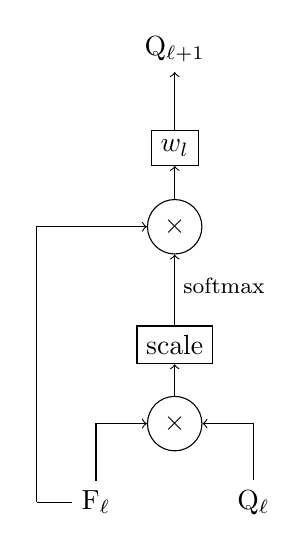
\begin{tikzpicture}
        \node (Q) at (4.5, -0.5) {Q$_\ell$};
        % \node (dimq) at (5, 0) {\scriptsize${1\times d_\ell}$};
        \node (F) at (2.5, -0.5) {F$_{\ell}$};
        % \node (dimft) at (3.0, -0) {\scriptsize${d_{\ell}\times p}$};
        \node (empt1) at (1.75, -0.5) {};
        \node[shape=circle,draw=black] (mm1) at (3.5, 0.5) {$\times$};
        % \node (dimraw) at (4,1) {\scriptsize$1\times p$};
        \node[shape=rectangle,draw=black](scale) at (3.5, 1.5) {scale};
        % \node (dimf) at (2.5, 3.175) {\scriptsize${p\times d_{\ell}}$};
        \node (soft) at (4.125, 2.25) {\footnotesize softmax};
        \node[shape=circle,draw=black] (mm2) at (3.5, 3) {$\times$};
        % \node[shape=rectangle,draw=black](project) at (3.5, 4) {$w_l: d_\ell\times d_{\ell+1}$ };
        \node[shape=rectangle,draw=black](project) at (3.5, 4) {$w_l$};
        % \node (dimscaled) [] at (4.25, 3.5) {\scriptsize $1\times d_\ell$};
        % \node [shape=circle,draw=black](sum1) at (3.5, 4) {+};
        % \node [shape=rectangle,draw=black](norm) at (3.5, 5.75) {LayerNorm};
        \node (Qplus1) at (3.5, 5.25) {Q$_{\ell+1}$};
        % \node (dimql) [align=left] at (4.25, 4.75) {\scriptsize$1\times d_{\ell+1}$};
        % \node (empt2) at (5.75, -0.5) {};

        \draw[->] (Q) |- node {} (mm1);
        \draw[->] (F) |- node {} (mm1);
        % \draw[-] (Q) -| node {} (empt2);
        % \draw[->] (empt2.center) |- node {} (sum1);
        \draw[->] (mm1) -- node {} (scale);
        \draw[->] (scale) -- node {} (mm2);
        \draw[-] (F) -| node {} (empt1.center);
        \draw[->] (empt1.center) |- node {} (mm2);
        \draw[->] (mm2) -- node {} (project);
        % \draw[->] (sum1) -- node {} (project);
        \draw[->] (project) -- node {} (Qplus1);
        % \draw[->] (norm) -- node {} (Qplus1);
    \end{tikzpicture}
    \caption{A Cross Attention Block. We denote matrix multiplication as "$\otimes$". The softmax operation is performed on each row). For a given layer $\ell$ we update our [CLS] token $Q_\ell$; by computing its scaled cross attention with the feature maps $F_\ell$, that are then projected to the channel dimension in the following stage, using a dense layer parametrized by $w_\ell$.}
    \label{fig:fig_crossatt}
\end{figure}

\section{Cross Attention Stream}
\label{sec:ca_design}
\input{fig/castream/ca_mainfig.tex}
\section{Experiments}
\label{sec:exp}

We evaluate the interpretability and recognition capabilities of our approach. In particular, we generate explanations following current state-of-the art post-hoc interpretability methods derived from CAM~\cite{zhou2016learning}. We compare the properties of the backbone network $f$ with and without our \Ours, where $f$ is pretrained and fixed.

\subsection{Experimental setup}
\label{subsec:setup}

\paragraph{Training}

We train and evaluate our models on the ImageNet ILSVRC-2012 dataset~\cite{deng2009imagenet}, on the training and validation splits respectively. Thus, we experiment with ResNet-based architectures~\cite{he2016deep} such as ResNet-18 and ResNet-50, and ConvNeXt based architectures~\cite{liu2022convnet} such as ConvNeXt-Small and ConvNeXt-Base. We aim at learning our \Ours, generating a \cls token that interacts with feature maps at different stages of network $f$, to serve as an attention-based pooling mechanism in order to interpret the predictions of $f$. Therefore, we experiment with pretrained models\footnote{https://pytorch.org/vision/0.8/models.html}, that we keep frozen while the parameters of the \Ours are optimized. Details on training hyperparameters are given in the appendix.

Moreover, we present experiments on the bird dataset: CUB-200-2011 \cite{WahCUB_200_2011} and on PASCAL VOC 2012 dataset \cite{Everingham15}. Here the ResNet-50 network is fine-tuned to these dataset as baseline. Then, our \Ours is learned as for ImageNet.

\paragraph{Evaluation}

We employ existing post-hoc interpretability methods to generate saliency maps with and without \Ours and compare interpretability metrics as well as classification accuracy. Regarding interpretability methods, we use Grad-CAM~\cite{DBLP:journals/corr/SelvarajuDVCPB16}, Grad-CAM++~\cite{DBLP:journals/corr/abs-1710-11063} and ScoreCAM~\cite{DBLP:journals/corr/abs-1910-01279}. We note that the evaluation is performed on the entire validation set, unlike the previous approaches.

Following Opti-CAM~\cite{zhang2023opti}, we use a number of classification metrics for interpretability. In particular, we consider the changes in predictive power measured by \emph{average drop} (AD)~\cite{DBLP:journals/corr/abs-1710-11063} and \emph{average gain} (AG)~\cite{zhang2023opti}, the proportion of better explanations measured by \emph{average increase} (AI)~\cite{DBLP:journals/corr/abs-1710-11063} and the impact of different extent of masking measured by \emph{insertion} (I) and \emph{deletion} (D)~\citep{petsiuk2018rise}.

% For localization, we use metrics from the \emph{weakly-supervised object localization} (WSOL) task to measure the maximum overlap between the saliency map (or corresponding predicted bounding boxes) and ground truth bounding boxes, \ie \emph{official metric} (OM), \emph{localization error} (LE), \emph{pixel-wise $F_1$ score}, \emph{box accuracy} (BoxAcc)~\citep{choe2020evaluating} and \emph{saliency metric} (SM)~\citep{dabkowski2017real}. We also measure the localization of the pixel of maximum saliency by the \emph{standard pointing game} (SP)~\cite{zhang2018top} and the fraction of the saliency map within the ground truth bounding boxes by \emph{energy pointing game} (EP)~\citep{DBLP:journals/corr/abs-1910-01279}. We obtain the ground truth bounding boxes from the ILSVRC2014\footnote{\url{https://www.image-net.org/challenges/LSVRC/2014/index\#}} dataset. 



%--------------------------------------------------------------------------------------------------
\section{Qualitative Results}
\label{sec:ca_qual}
\subsection{Qualitative evaluation}
\label{subsec:vinspection}    
We show saliency maps obtained by different interpretability methods using either \gap or \Ours, as 
well as the class-agnostic raw attention coming from our \Ours, see \autoref{fig:compmethods}.\\
%--------------------------------------------------------------------------------------------------
\begin{figure}[H]
    \scriptsize
    \centering
    \setlength{\tabcolsep}{1.5pt}
    % \resizebox{\textwidth}{!}{%
    \begin{tabular}{ccccccccc}
        {}&\multirow{2}{*}{Input image}&\multirow{2}{*}{Raw Attention}&\multicolumn{2}{c}{Grad-CAM}&\multicolumn{2}{c}{Grad-CAM++}&\multicolumn{1}{c}{Score-CAM}\\
        {}&{}&{}&GAP&\Ours&GAP&\Ours&GAP&\Ours\\   
        {\rotatebox{90}{\tiny Envelope}}&\includegraphics[width=0.115\textwidth]{fig/castream/images/Comparable/figure1_similarities/original/23541.jpeg}&\includegraphics[width=0.115\textwidth]{fig/castream/images/Comparable/figure1_similarities/raw_att/23541.jpeg}&\includegraphics[width=0.115\textwidth]{fig/castream/images/Comparable/figure1_similarities/shelf_gradcam/23541.jpeg}&\includegraphics[width=0.115\textwidth]{fig/castream/images/Comparable/figure1_similarities/gradcam/23541.jpeg}&\includegraphics[width=0.115\textwidth]{fig/castream/images/Comparable/figure1_similarities/shelf_gradcampp/23541.jpeg}&\includegraphics[width=0.115\textwidth]{fig/castream/images/Comparable/figure1_similarities/gradcampp/23541.jpeg}&\includegraphics[width=0.115\textwidth]{fig/castream/images/Comparable/figure1_similarities/scorecam/23541.jpeg}&\includegraphics[width=0.115\textwidth]{fig/castream/images/Comparable/figure1_similarities/shelf_scorecam/23541.jpeg}\\
        {\rotatebox{90}{\tiny Groom}}&\includegraphics[width=0.115\textwidth]{fig/castream/images/Comparable/figure1_similarities/original/9602.jpeg}&\includegraphics[width=0.115\textwidth]{fig/castream/images/Comparable/figure1_similarities/raw_att/9602.jpeg}&\includegraphics[width=0.115\textwidth]{fig/castream/images/Comparable/figure1_similarities/shelf_gradcam/9602.jpeg}&\includegraphics[width=0.115\textwidth]{fig/castream/images/Comparable/figure1_similarities/gradcam/9602.jpeg}&\includegraphics[width=0.115\textwidth]{fig/castream/images/Comparable/figure1_similarities/shelf_gradcampp/9602.jpeg}&\includegraphics[width=0.115\textwidth]{fig/castream/images/Comparable/figure1_similarities/gradcampp/9602.jpeg}&\includegraphics[width=0.115\textwidth]{fig/castream/images/Comparable/figure1_similarities/scorecam/9602.jpeg}&\includegraphics[width=0.115\textwidth]{fig/castream/images/Comparable/figure1_similarities/shelf_scorecam/9602.jpeg}\\    
        {\rotatebox{90}{\tiny Nematode}}&\includegraphics[width=0.115\textwidth]{fig/castream/images/Comparable/figure1_similarities/original/12414.jpeg}&\includegraphics[width=0.115\textwidth]{fig/castream/images/Comparable/figure1_similarities/raw_att/12414.jpeg}&\includegraphics[width=0.115\textwidth]{fig/castream/images/Comparable/figure1_similarities/shelf_gradcam/12414.jpeg}&\includegraphics[width=0.115\textwidth]{fig/castream/images/Comparable/figure1_similarities/gradcam/12414.jpeg}&\includegraphics[width=0.115\textwidth]{fig/castream/images/Comparable/figure1_similarities/shelf_gradcampp/12414.jpeg}&\includegraphics[width=0.115\textwidth]{fig/castream/images/Comparable/figure1_similarities/gradcampp/12414.jpeg}&\includegraphics[width=0.115\textwidth]{fig/castream/images/Comparable/figure1_similarities/scorecam/12414.jpeg}&\includegraphics[width=0.115\textwidth]{fig/castream/images/Comparable/figure1_similarities/shelf_scorecam/12414.jpeg}\\
        {\rotatebox{90}{\tiny CRT screen}}&\multicolumn{1}{c}{\includegraphics[width=0.115\textwidth]{fig/castream/images/Comparable/figure1/original/43057.jpeg}}&\multicolumn{1}{c}{\includegraphics[width=0.115\textwidth]{fig/castream/images/Comparable/figure1/raw_att/43057.jpeg}}&\multicolumn{1}{c}{\includegraphics[width=0.115\textwidth]{fig/castream/images/Comparable/figure1/shelf_gradcam/43057.jpeg}}&\multicolumn{1}{c}{\includegraphics[width=0.115\textwidth]{fig/castream/images/Comparable/figure1/gradcam/43057.jpeg}}&\multicolumn{1}{c}{\includegraphics[width=0.115\textwidth]{fig/castream/images/Comparable/figure1/shelf_gradcampp/43057.jpeg}}&\multicolumn{1}{c}{\includegraphics[width=0.115\textwidth]{fig/castream/images/Comparable/figure1/gradcampp/43057.jpeg}}&\multicolumn{1}{c}{\includegraphics[width=0.115\textwidth]{fig/castream/images/Comparable/figure1/shelf_scorecam/43057.jpeg}}&\multicolumn{1}{c}{\includegraphics[width=0.115\textwidth]{fig/castream/images/Comparable/figure1/scorecam/43057.jpeg}}\\ % Checked     
        {\rotatebox{90}{\tiny Snowboard}}&\includegraphics[width=0.115\textwidth]{fig/castream/images/Comparable/figure1_similarities/original/11376.jpeg}&\includegraphics[width=0.115\textwidth]{fig/castream/images/Comparable/figure1_similarities/raw_att/11376.jpeg}&\includegraphics[width=0.115\textwidth]{fig/castream/images/Comparable/figure1_similarities/shelf_gradcam/11376.jpeg}&\includegraphics[width=0.115\textwidth]{fig/castream/images/Comparable/figure1_similarities/gradcam/11376.jpeg}&\includegraphics[width=0.115\textwidth]{fig/castream/images/Comparable/figure1_similarities/shelf_gradcampp/11376.jpeg}&\includegraphics[width=0.115\textwidth]{fig/castream/images/Comparable/figure1_similarities/gradcampp/11376.jpeg}&\includegraphics[width=0.115\textwidth]{fig/castream/images/Comparable/figure1_similarities/scorecam/11376.jpeg}&\includegraphics[width=0.115\textwidth]{fig/castream/images/Comparable/figure1_similarities/shelf_scorecam/11376.jpeg}\\   
    \end{tabular}
    % }
    \vspace{3pt}
    \caption{}
    %Comparison of saliency maps generated by different CAM-based methods, using GAP and our \Ours, on ImageNet images. The raw attention is the one used for pooling by \Ours.
    \label{fig:compmethods}
    \end{figure}

We observe that the raw attention focuses on objects of interest in the images. 
In general, saliency maps obtained with \Ours are similar but tend to cover larger regions of the 
object or more instances compared with \gap.\\
\begin{figure}[t]
\scriptsize
\centering
\setlength{\tabcolsep}{1.3pt}
%    \resizebox{\columnwidth}{!}{%
     \begin{tabular}{cccccccc}
           \mc{2}{Corridor}&\mc{2}{Greenhouse}&\mc{2}{Pool Inside}&\mc{2}{Wine Cellar}\\
           Input image&Raw Attention&Input image&Raw Attention&Input image&Raw Attention&Input image&Raw Attention\\
           \includegraphics[width=0.12\textwidth,height=0.08\textwidth]{fig/castream/images/Outdataset/Corridor/Original/c1.jpg}&
           \includegraphics[width=0.12\textwidth,height=0.08\textwidth]{fig/castream/images/Outdataset/Corridor/Attention/c1.jpg}&
           \includegraphics[width=0.12\textwidth,height=0.08\textwidth]{fig/castream/images/Outdataset/Greenhouse/Original/celosie_02.jpg}&
           \includegraphics[width=0.12\textwidth,height=0.08\textwidth]{fig/castream/images/Outdataset/Greenhouse/Attention/celosie_02.jpg}&
           \includegraphics[width=0.12\textwidth,height=0.08\textwidth]{fig/castream/images/Outdataset/Poolinside/Original/003_1b.jpg}&
           \includegraphics[width=0.12\textwidth,height=0.08\textwidth]{fig/castream/images/Outdataset/Poolinside/Attention/003_1b.jpg}&
           \includegraphics[width=0.12\textwidth,height=0.08\textwidth]{fig/castream/images/Outdataset/WineCellar/Original/bodega2.jpg}&
           \includegraphics[width=0.12\textwidth,height=0.08\textwidth]{fig/castream/images/Outdataset/WineCellar/Attention/bodega2.jpg}\\
           
           \includegraphics[width=0.12\textwidth,height=0.08\textwidth]{fig/castream/images/Outdataset/Corridor/Original/1L_10_Corridor_A.jpg}&
           \includegraphics[width=0.12\textwidth,height=0.08\textwidth]{fig/castream/images/Outdataset/Corridor/Attention/1L_10_Corridor_A.jpg}&
           \includegraphics[width=0.12\textwidth,height=0.08\textwidth]{fig/castream/images/Outdataset/Greenhouse/Original/20070417klpcnatun_229_Ies_SCO.jpg}&
           \includegraphics[width=0.12\textwidth,height=0.08\textwidth]{fig/castream/images/Outdataset/Greenhouse/Attention/20070417klpcnatun_229_Ies_SCO.jpg}&
           \includegraphics[width=0.12\textwidth,height=0.08\textwidth]{fig/castream/images/Outdataset/Poolinside/Original/141821195_M.jpg}&
           \includegraphics[width=0.12\textwidth,height=0.08\textwidth]{fig/castream/images/Outdataset/Poolinside/Attention/141821195_M.jpg}&
           \includegraphics[width=0.12\textwidth,height=0.08\textwidth]{fig/castream/images/Outdataset/WineCellar/Original/bodega_45_18_yahoo.jpg}&
           \includegraphics[width=0.12\textwidth,height=0.08\textwidth]{fig/castream/images/Outdataset/WineCellar/Attention/bodega_45_18_yahoo.jpg}\\
           
           \includegraphics[width=0.12\textwidth,height=0.08\textwidth]{fig/castream/images/Outdataset/Corridor/Original/430_Korridor_300.jpg}&
           \includegraphics[width=0.12\textwidth,height=0.08\textwidth]{fig/castream/images/Outdataset/Corridor/Attention/430_Korridor_300.jpg}&
           \includegraphics[width=0.12\textwidth,height=0.08\textwidth]{fig/castream/images/Outdataset/Greenhouse/Original/20070418klpcnaecl_364_Ies_SCO.jpg}&
           \includegraphics[width=0.12\textwidth,height=0.08\textwidth]{fig/castream/images/Outdataset/Greenhouse/Attention/20070418klpcnaecl_364_Ies_SCO.jpg}&
           \includegraphics[width=0.12\textwidth,height=0.08\textwidth]{fig/castream/images/Outdataset/Poolinside/Original/catalogue_piscine_interieur.jpg}&
           \includegraphics[width=0.12\textwidth,height=0.08\textwidth]{fig/castream/images/Outdataset/Poolinside/Attention/catalogue_piscine_interieur.jpg}&
           \includegraphics[width=0.12\textwidth,height=0.08\textwidth]{fig/castream/images/Outdataset/WineCellar/Original/bodega_63_24_flickr.jpg}&
           \includegraphics[width=0.12\textwidth,height=0.08\textwidth]{fig/castream/images/Outdataset/WineCellar/Attention/bodega_63_24_flickr.jpg}\\
           
           \includegraphics[width=0.12\textwidth,height=0.08\textwidth]{fig/castream/images/Outdataset/Corridor/Original/06_Right_corridor_of_the_main_hall.jpg}&
           \includegraphics[width=0.12\textwidth,height=0.08\textwidth]{fig/castream/images/Outdataset/Corridor/Attention/06_Right_corridor_of_the_main_hall.jpg}&
           \includegraphics[width=0.12\textwidth,height=0.08\textwidth]{fig/castream/images/Outdataset/Greenhouse/Original/2026_2006_Grimm_s_Gardens_Greenhouse.jpg}&
           \includegraphics[width=0.12\textwidth,height=0.08\textwidth]{fig/castream/images/Outdataset/Greenhouse/Attention/2026_2006_Grimm_s_Gardens_Greenhouse.jpg}&
           \includegraphics[width=0.12\textwidth,height=0.08\textwidth]{fig/castream/images/Outdataset/Poolinside/Original/connolly_center_pool_inside_lg.jpg}&
           \includegraphics[width=0.12\textwidth,height=0.08\textwidth]{fig/castream/images/Outdataset/Poolinside/Attention/connolly_center_pool_inside_lg.jpg}&
           \includegraphics[width=0.12\textwidth,height=0.08\textwidth]{fig/castream/images/Outdataset/WineCellar/Original/bodega_78_08_flickr.jpg}&
           \includegraphics[width=0.12\textwidth,height=0.08\textwidth]{fig/castream/images/Outdataset/WineCellar/Attention/bodega_78_08_flickr.jpg}\\              
    \end{tabular}
%    }
    \vspace{3pt}
    \caption{\textbf{Raw attention maps} obtained from our \Ours on images of the MIT 67 Scenes dataset \autocite{quattoni2009recognizing} on classes that do not exist in ImageNet. The network sees them at inference for the first time.} 
    %
    \label{fig:enter-label}
\end{figure}  
Indeed, the differences in saliency maps should not be large, as both methods share the same 
features maps $F^k_\ell$ and only the weight coefficients $\alpha^c_k$ differ.
Despite the small differences, the following quantitative results show that \Ours has a significant 
impact on the interpretability metrics.
   
In addition, \autoref{fig:enter-label} shows examples of images from the MIT 67 Scenes 
dataset \autocite{quattoni2009recognizing} along with raw attention maps obtained by \Ours. These 
images come from four classes that do not exist in ImageNet and the network sees them at inference for 
the first time. Nevertheless, the attention maps focus on objects of interest in general.

\section{Quantitative Results}
\label{sec:ca_quant}

\newpage


	\chapter{Zero Information in Interpretability}
\chaptertoc{}
\label{ch:zip}
\section{ZIP definition}
\label{sec:zip_algo}

\section{Extension: Insertion-Deletion}
\label{sec:zip_insdel}

\section{Qualitative Evaluation}
\label{sec:zip_qual}

\section{Benchmark}
\label{sec:zip_benchmark}

	%--------------------------------------------------------------------------------------------------
\addchap{Conclusion}
%\addcontentsline{toc}{chapter}{Conclusion}
\label{concs}
Across this thesis we studied explainable deep learning proposals, to understand image 
recognition models. Explainable Artificial Intelligence and Interpretability are blooming fields 
within the research community. In particular, current high performing models are 
being steadily assimilated within society and their prominence in human life is increasing. Thus, 
it is important to understand the processes prompting a prediction in such models. 
Furthermore, these fields are being studied following a plethora of axis of research. Still, the 
work presented by Lipton \autocite{mythos_interp} and Zhang \autocite{zhang2021survey} lay the 
foundation for our work.\\

We structure these conclusions of our work in the following manner. First on \autoref{sec:conc_gen} 
we comment on the thesis objectives and the manner they were addressed across each chapter. On 
\autoref{sec:conc_futur} we address future work regarding this topic.\\

\section{General remarks}
\label{sec:conc_gen}
%In this section, we describe each chapter's contributions and general observations. To begin 
%with, \autoref{sub:conc_obj} elaborates on the overall objectives and the work conducted in this 
%thesis. In more detail, \autoref{sub:conc_back} raises conclusions regarding the background, 
%advancements in current image recognition techniques, and the need for interpretability. Then, 
%\autoref{sub:conc_opti} discusses interpretability evaluation issues and how we address them with 
%our proposal. Later, on \autoref{sub:conc_ca} the conclusion follows the Cross Attention Stream 
%proposal to improve explanations. Lastly, \autoref{sub:conc_grad} summarizes the outcome of 
%the gradient denoising chapter.

\paragraph{Thesis Objectives}
\label{sub:conc_obj}
This thesis was conducted to study image recognition models, building novel explainability 
approaches to further understand them. In detail, our major objective was to improve both 
recognition and interpretability properties. To that end, we identified three areas of  
work: high computational cost, lack of consensus between evaluation procedures, and a mismatch 
between human and model interpretability.\\

\noindent To begin with, regarding the improvement of image recognition, this work 
introduced two different approaches that address this requirement. In particular, Chapter 
\ref{ch:castream} showcased how the addition of cross attention can enhance 
recognition characteristics. Furthermore, Chapter \ref{ch:grad} presented a novel training 
paradigm that can potentially yield better recognition predictions. Complementary to this, 
interpretability measurements are improved consistently across this thesis. In particular, 
Chapter \ref{ch:opticam} presented \emph{Opti-CAM}, a methodology that consistently improves 
upon these capabilities, evidenced across different datasets and evaluation modes: 
recognition and localization.\\

\noindent In line with the specific objectives, our thesis follows a standardized evaluation 
procedure. Across each chapter, we compare baselines with our approaches under the exact 
same settings. Conversely, we observed limitations in the details of the evaluation of 
xAI methodologies. We hope that our contributions will encourage the community towards a 
set of good practices in this domain.\\

\noindent Lastly, the differences between human and model interpretations were discussed in 
detail in Chapter \ref{ch:opticam}. Specifically, we observed that context matters in the 
formulation of saliency maps: the most important regions describing a category are spread across 
the image. This is highlighted with the failure on interpretable object localization, and the 
success on interpretable object recognition achieved by Opti-CAM: human centric explanations 
expect the most salient areas to be found mostly over the object of interest. \\

\paragraph{Background}
\label{sub:conc_back}
\noindent In Chapter \ref{ch:rel}, we introduced and described the evolution of image recognition 
models. We started with models based on traditional machine learning algorithms, to current high 
performance architectures based on attention computation. In relation to this modelling evolution, we 
demonstrated how the improvement of image recognition models consequently benefits the development 
of related Computer Vision fundamental tasks. Thus, further development of image recognition models 
is acknowledged as a major task in Computer Vision, enhancing adjacent tasks within the discipline.\\

\noindent Complementary to the introduction of these models, we highlighted the 
necessity of providing explanations to current image recognition models. We mentioned the proposition  
of the European AI act to regulate Artificial Intelligence technologies, as well as in the 
Mythos of Model Interpretability by Lipton. In particular, following Lipton's work we 
revised the properties proposed therein, as well as illustrated how they can be adapted to explain 
current state-of-the-art models. Furthermore, we demonstrated our interest on \gls{cam} methods 
to produce explanations. A thorough description of their computation and different proposals is 
established to lay the foundation for the following studies.\\

\noindent Finally, we also introduced evaluation methods to assess the effect of the attribution 
methods mentioned. Regarding these evaluation procedures, we grouped 
them according to the reasoning of the measurement provided, as well as highlighted the positive 
and negative points of each procedure. Notably, Interpretable Object Recognition and 
Causal Analysis are observed to best assess interpertability properties of a model. On one 
hand, it is observed that Interpretable Object Localization implies that model 
interpretations should be aligned with human interpretations. On the other hand, pure human 
measurements are completely aligned with what individuals deem salient on images, which is often 
biased and not replicable on experimental settings. Pure classifier centric evaluation 
ultimately addresses these shortcomings, removing implicit bias produced by human reasoning, 
although not from supervision.\\

\paragraph{Opti-CAM}
\label{sub:conc_opti}
\noindent Chapter \ref{ch:opticam} presented our first contribution: Opti-CAM, a post-hoc 
interpretability method, constructed following the principles of CAM and evaluation 
procedures. Specifically, Opti-CAM produces a saliency map that maximizes predictive probability 
of images masked by it. Additionally, issues regarding quantitative evaluation are displayed, 
most importantly the incompleteness of \textbf{Interpretable Object Recognition}. To address these 
shortcomings, we proposed Average Gain, a complementary metric to Average Drop, measuring 
the predictive gains obtained while considering explanation maps as input images.\\

\noindent On one hand, we observed that true to its design, Opti-CAM outperforms contemporary 
CAM attribution methods in most quantitative measurements. In particular, this methodology 
performs the best in \textbf{Interpretable Image Recognition} and \textbf{Causal Analysis}, but 
fails in \textbf{Object Localization}. We made sense of these observations aided with 
visualizations. In contrast to current CAM methods, Opti-CAM generates a saliency map that is 
spread across the input image. From this we infer that context matters describing an explanation. 
Consequently, since context is necessary to explain a prediction, the requirement of saliency maps 
covering the object of interest, is counter-intuitive and does not hold.\\

\noindent Lastly, regarding Average Gain our experimental results demonstrated its complementary 
behavior to Interpretable Image Recognition Evaluation.  In particular, this metric efficiently 
demonstrates how Fake-CAM fails as an attribution method: although it attains almost perfect 
Average Drop; its Average Gain measurement fails entirely, effectively complementing the 
shortcomings instated by this CAM method. Still, a complete benchmark comparing most attribution 
methods, as well as explanations for predicted labels, would provide a reality check on the 
evaluation of interpretability\\

\paragraph{Cross-Attention Stream}
\label{sub:conc_ca}
\noindent Chapter \ref{ch:castream} presented our second contribution, the Cross-Attention Stream. 
This addition inspired by pure attention architectures, computes an abstract representation of 
classes, via interaction of a class token and feature maps across different depths of a model. 
Additionally, this approach was validated in common image recognition models studied on 
interpretability such as ResNet, as well as in a family of models not often studied in this fashion: 
ConvNeXt.\\

\noindent In this chapter, we set the stage for quantitative interpretability measurements for 
transparency based approaches. We trained the stream similarly to prior transparency approaches, 
and we evaluated its properties using \gls{cam}, a post-hoc method. Moreover, we observed that our 
saliency maps do not differ much from the baseline ones. However, this result was expected as this 
approach does not modify existing parameters within the network, nor changes the computation of 
attributions. Instead, our representation conveys information differently to the classifier, 
enhancing predicted probability of groundtruth classes. \\

\paragraph{Gradient Denoising}
\label{sub:conc_grad}
\noindent Lastly, Chapter \ref{ch:grad} introduced a learning paradigm for interpretable gradients. 
In this approach, the guided backpropagated gradient of the network, observed in the input space is 
used to regularize the network gradient during training, enhancing interpretability properties. 
Continuing with the evaluation of transparency methods seen on Chapter \ref{ch:castream}, we 
evaluate these properties using CAM methods.\\

\noindent From the family of pure gradient based attribution methods, guided 
backpropagation required less computation to function. In stark contrast with approaches such as 
smooth gradients and integrated gradients, guided backpropagation maintains the requirement of 
one forward pass and one backward through the model to generate an output.\\

\noindent Lastly, we observed that pure guided backpropagation training is not plausible. During 
the prototyping phase of this chapter, we experimented using this setting, and we found that 
the training was unstable leading to gradients pushing towards infinity. We hypothesize that 
gradient information produced by responses to negative gradients, regularizes neural network 
training.\\

\section{Future Work}
\label{sec:conc_futur}
We set the foundation for our future work in three axes. First, a discussion on the future for 
interpretable image recognition. Then, we iterate over how our proposals can be 
improved upon in the future. Finally, exploratory directions beyond the scope of this thesis.\\

\paragraph{Interpretable Image Recognition}
The development of image recognition models within computer vision and deep learning benefits 
from ongoing advancements. With the recent emergence of CNNs and transformers, new architectures 
are expected to continue appearing. Evaluating the impact of these models through testing and 
proposing methodologies is essential for future progress. While CNNs have been extensively 
studied over the past decade, the properties and functioning of transformers remain an open field. 
Despite transformers being newer, their impact and performance are significant, necessitating 
further study. However, research on CNNs should also continue.\\

\noindent Additionally, standardization of interpretability study and evaluation is another area 
with potential for future work. A thorough differentiation between model 
interpretability and human interpretability studies should be established. A preliminary study 
regarding this topic is conducted in this thesis, still a widespread adoption within the 
community is mostly desired. To achieve this, a more thorough survey describing these comparisons, 
as well as the failure of current interpretability evaluation methods is one manner to address 
these requirements.\\

\paragraph{On the chapters of this thesis}
\noindent Regarding Opti-CAM, we observe one possibility for future work. CAM-based 
attributions struggle to explain transformer-based architectures. These saliency maps are often 
sparse and do not provide sufficient clarity when compared to raw attention. A different 
attribution method could provide improved representations, possibly calculated using the class 
token. Accounting for the fixation of saliency maps on transformers as demonstrated on 
Simpool \autocite{psomas2023simpool} and Registers \autocite{darcet2024vision} would 
allow for updates of this approach or a novel attribution method.\\

\noindent On the topic of Cross-Attention, future work aims at optimizing the architecture and 
broadening its scope to different models. In particular, the parameter count can be reduced by 
shortening the stream length, focusing only on layers where semantic information is prominent. 
Additionally, expanding beyond the usage of ResNet and ConvNeXt, and presenting an optimized 
training paradigm for this approach, would enable its application to more architectures, enhancing 
its coverage of image recognition tasks.\\

\noindent Lastly, the gradient denoising paradigm was showcased in a constrained setting: small 
datasets and low-parameter networks. This limitation is due to the high computational cost of the 
approach. However, the promising results suggest that addressing this complexity could allow for 
scaling to large-scale image datasets and more complex models.\\

\paragraph{Beyond the scope of this thesis}
Currently, computer vision is one open field, thriving with possibilities for further research 
and industry developments. In particular, during the development of this thesis several 
technologies were unveiled, addressing different areas of study for artificial intelligence. 
For instance, \gls{nlp} is currently a prominent field where technologies like Large Language 
Models have taken the spotlight. However, such kind of developments require heavy computational 
infrastructure, limiting their development to bigger research groups. Optimizing such methodologies, 
as well as producing competitive, yet more simplified alternatives is one path where research 
could be focused as well.\\

\noindent In contrast to developing large models and mainstream tasks, future work could focus on 
updating particular applications. Concepts from general image recognition and interpretability are 
applied to fields such as medical diagnosis and industry, requiring highly specific models. 
Adapting and modifying state-of-the-art models for these fine-grained applications is a key 
direction for future developments.\\

\noindent Lastly, on a personal level, future work comprises on setting the stage for continuing a 
scientific career. To achieve this, I aim to continue with a post-doctoral position on topics 
aligned with my interests: image recognition, explainable AI and foundational models. Moreover, 
given my focus on academia, pursuing a research engineer position is a direction  that would 
also allow to advance for my career.

    %\appendix

	\newpage
	\printbibliography[heading=bibintoc]%% bibliographie
	
	%\newpage
	%\printindex							%% index
	
	%\newpage
	%\printendnotes						%% notes

	%\input{tex_append/annexes}			%% annexes

\end{document}
